% !TeX encoding = UTF-8
% !TeX program = xelatex
% !TeX spellcheck = en_US

\documentclass[degree=master,fontset=mac]{sysuthesis 2}
% degree      = doctor | master | bachelor
% degree-type = academic | professional
% language    = chinese | english
% fontset     = windows | mac | ubuntu | fandol

\makeatletter
\newif\ifsysu@math@style@TeX
\sysu@math@style@TeXfalse
\define@key{sysu}{title}{\ctitle{#1}}
\define@key{sysu}{title*}{\etitle{#1}}
\define@key{sysu}{author}{\cauthor{#1}}
\define@key{sysu}{author*}{\eauthor{#1}}
\define@key{sysu}{speciality}{\cmajor{#1}}
\define@key{sysu}{speciality*}{\emajor{#1}}
\define@key{sysu}{supervisor}{\cmentor{#1}}
\define@key{sysu}{supervisor*}{\ementor{#1}}
\define@key{sysu}{practice-supervisor}{\cindustrymentor{#1}}
\define@key{sysu}{practice-supervisor*}{\cindustrymentor{#1}}
\define@key{sysu}{keywords}{\ckeywords{#1}}
\define@key{sysu}{keywords*}{\ekeywords{#1}}
\define@key{sysu}{math-style}{}
\define@key{sysu}{math-font}{}
\define@key{sysu}{cite-style}{}
\define@key{sysu}{professional-type}{}
\define@key{sysu}{professional-type*}{}
\define@key{sysu}{department}{}
\define@key{sysu}{student-id}{}
\define@key{sysu}{secret-level}{}
\define@key{sysu}{secret-level*}{}
\define@key{sysu}{secret-year}{}
\define@key{sysu}{reviewer}{}
\define@key{sysu}{date}{}
\eauthor{}
\emajor{}
\ementor{}
\cindustrymentor{}
\newcommand{\sysusetup}[1]{\setkeys{sysu}{#1}}
\let\copyrightpage\relax
\renewcommand{\bibsection}{%
	\chapter*{参考文献}%
	\addcontentsline{toc}{chapter}{参考文献}%
	\markboth{参考文献}{参考文献}%
}
\makeatother

% 加载宏包、全部的配置
% !TeX root = ./main.tex

\sysusetup{
  title                = {基于线图的非加性最短路径问题与GPU并行优化},
  title*               = {Line-Graph-Based Non-Additive Shortest Path Problems and GPU Parallel Optimization},
  speciality           = {应用统计},
  speciality*          = {Applied Statistics},
  % practice-supervisor  = {XXX~教授, XXX~教授},
  % practice-supervisor* = {Prof. XXX, Prof. XXX},
  % date                 = {2017-05-01},  % 完成时间，默认为今日
  % professional-type    = {专业学位类型},
  % professional-type*   = {Professional degree type},
  % department           = {学院/系（待填写）},  % 院系，本科生需要填写
  % student-id           = {学号（待填写）},      % 学号，本科生需要填写
  % secret-level         = {秘密},     % 绝密|机密|秘密|控阅，注释本行则公开
  % secret-level*        = {Secret},  % Top secret | Highly secret | Secret
  % secret-year          = {10},      % 保密/控阅期限
  % reviewer             = true,      % 声明页显示“评审专家签名”
  %
  % 数学字体
  % math-style           = GB,  % 可选：GB, TeX, ISO
  math-font            = xits,  % 可选：stix, xits, libertinus
  cite-style           = super,
}

%\renewcommand{\thefigure}{\thechapter-\arabic{figure}}% 将正文和目录的图片标题由x.x改为x-x，慎用
%\renewcommand{\thetable}{\arabic{chapter}-\arabic{table}}% 将正文和目录的表格标题由x.x改为x-x，慎用
%\renewcommand{\theequation}{\arabic{chapter}-\arabic{equation}}% 将正文的公式序号由(x.x)改为(x-x)，慎用

% 加载宏包

% 定理类环境宏包
\usepackage{amsthm}

% 中英文双标题
\usepackage{bicaption}

% 表注
\usepackage{threeparttable}

% 跨页表格
\usepackage{longtable}

% 绘图
\usepackage{tikz}
\usetikzlibrary{arrows.meta,positioning,matrix}

% 算法
\usepackage{float}
\usepackage[ruled,linesnumbered]{algorithm2e}
%\renewcommand{\thealgocf}{\arabic{chapter}-\arabic{algocf}}% 将算法标题由x.x改为x-x，慎用

% SI 量和单位
\usepackage{siunitx}

% 参考文献使用 BibTeX + natbib 宏包
% 顺序编码制
\usepackage[sort]{natbib}
\bibliographystyle{sysuthesis-numerical}

% 参考文献使用 BibLaTeX 宏包
% \usepackage[style=sysuthesis-numeric]{biblatex}
% 声明 BibLaTeX 的数据库
% \addbibresource{reference.bib}

% 配置图片的默认目录
\graphicspath{{figures/}}

% 数学命令
\makeatletter
\newcommand\dif{%  % 微分符号
  \mathop{}\!%
  \ifsysu@math@style@TeX
    d%
  \else
    \mathrm{d}%
  \fi
}
\makeatother
\newcommand\eu{{\symup{e}}}
\newcommand\iu{{\symup{i}}}

% 用于写文档的命令
\DeclareRobustCommand\cs[1]{\texttt{\char`\\#1}}
\DeclareRobustCommand\env[1]{\texttt{#1}}
\DeclareRobustCommand\pkg[1]{\textsf{#1}}
\DeclareRobustCommand\file[1]{\nolinkurl{#1}}

% hyperref 宏包在最后调用
\usepackage{hyperref}



\begin{document}

\maketitle
\copyrightpage

\frontmatter
% !TeX root = ../main.tex

\ckeywords{路径依赖最短路径, 有限阶历史依赖, 线图, 条件权重最短路径, GPU并行}
\ekeywords{Path-dependent shortest path, Finite-order history dependency, Line graph, Conditional Weighting Shortest Path, GPU parallelization}

\cabstract{
最短路径问题广泛应用于交通导航、物流调度与机器人规划等场景.传统最短路径模型默认边权可加且与路径历史无关，因而难以直接处理转向惩罚、禁转约束等由边间过渡关系诱发的路径依赖代价.针对该类有限阶历史依赖的非加性最短路径问题，本文构建了基于线图映射与条件加权的条件权重最短路径（Conditional Weighting Shortest Path, CWSP）框架，并围绕“拓扑替代构造-条件权重计算-替代图寻优”三阶段给出 GPU 并行化实现.

在建模层面，本文基于 $k$-加性思想将原图中的历史依赖状态显式展开为替代图节点，将动态转移代价静态编码为替代图边权，从而把原问题等价转化为加性最短路径问题，并给出最优性等价论证.在实现层面，针对线图化带来的规模膨胀与串行瓶颈，本文在阶段1采用“出度统计+并行前缀和+CSR 无锁写入”的并行构图策略，在阶段2采用边级并发与访存规整的条件加权策略，在阶段3采用桶式 $\Delta$-Stepping 算法替代全序优先队列 Dijkstra，以提升大规模场景下的整体吞吐能力.

实验在真实 MIA 微观滑行路网与多组网格数据上展开.结果显示：在 40 组带锐角惩罚的复杂点对测试中，传统 Dijkstra 成功率为 50\%，而 CWSP 成功率为 100\%.在规模扩展实验中，当线图规模达到 $|E_H|=1{,}431{,}608$ 时，端到端耗时由 CPU 的 $84.283\,$ms 降至 GPU 的 $17.276\,$ms，加速比达 $4.88\times$.进一步的历史阶数扩展实验（$k=1\sim5$）表明，随着状态空间膨胀，GPU 端到端加速比由 $2.29\times$ 提升至 $152.44\times$；当 $k=6$ 时出现显存不足，揭示了高阶场景下替代图构建与存储的资源上限问题.上述结果验证了本文方法在路径依赖建模正确性与并行可扩展性两方面的有效性.
}

\eabstract{
The shortest path problem is a fundamental problem in graph optimization and is widely used in transportation, logistics, and robotic planning. Classical shortest-path models assume additive edge costs independent of path history, which makes them inadequate for path-dependent settings such as turn penalties and prohibited turns. To address finite-order history-dependent non-additive shortest path problems, this thesis develops a Conditional Weighting Shortest Path (CWSP) framework based on line-graph transformation, and implements a three-stage GPU pipeline: topology substitution, conditional weighting, and shortest-path search on the transformed graph.

From the modeling perspective, the proposed method uses the $k$-additive formulation to explicitly encode history-dependent states as nodes in an alternative graph and converts dynamic transition costs into static edge weights. This transformation reduces the original non-additive problem to an additive shortest-path problem with preserved optimality. From the implementation perspective, to mitigate graph-size inflation and serial bottlenecks, stage 1 adopts parallel out-degree counting, prefix-sum allocation, and lock-free CSR filling; stage 2 applies edge-level parallel conditional weighting with memory-access regularization; stage 3 replaces globally ordered priority-queue Dijkstra with bucket-based $\Delta$-Stepping algorithm to increase parallel relaxation throughput.

Experiments are conducted on the real Miami International Airport (MIA) taxiway network and multiple grid datasets. On 40 constrained origin-destination pairs with sharp-turn penalties, traditional Dijkstra achieves only a 50\% success rate, while CWSP achieves 100\%. In large-scale tests, when the transformed graph reaches $|E_H|=1{,}431{,}608$, end-to-end runtime is reduced from $84.283$ ms on CPU to $17.276$ ms on GPU, yielding a $4.88\times$ speedup. In higher-order history experiments ($k=1\sim5$), end-to-end GPU speedup increases from $2.29\times$ to $152.44\times$ as state-space expansion grows. An out-of-memory event at $k=6$ further indicates that graph construction and storage become the primary resource bottleneck in high-order scenarios. These results demonstrate both the modeling validity and the parallel scalability of the proposed approach.
}

\makeabstract

\tableofcontents
% \listoffiguresandtables
% % !TeX root = ../main.tex

% 符号表（如不需要可保持为空，或在 main.tex 中注释掉对应 \input）
%\begin{notation}
%  \begin{notationlist}{2em}
%    \item[$a$] 含义
%  \end{notationlist}
%\end{notation}


\mainmatter
% !TeX root = ../main.tex

\chapter{绪论}

\section{研究背景及意义}

\section{国内外研究现状}

\section{本文研究内容}

\section{后续章节安排}


% !TeX root = ../main.tex

\chapter{非加性最短路径问题及其算法}

本章主要围绕非加性最短路径问题的基本概念、典型特征及其求解方法展开论述.首先介绍图的基本定义及常见存储方式，为后续算法描述统一符号体系和数据结构基础；其次回顾经典最短路径问题的定义及其基本求解算法，说明传统最短路径模型成立所依赖的加性假设；然后在此基础上给出非加性最短路径问题的形式化定义、主要类别以及路径依赖型问题的经典求解思路，并分析传统算法在该类问题中失效的根本原因；接着介绍线图理论的基本概念及其在路径依赖建模中的作用；最后对 CUDA 并行框架进行简要说明，为下一章的算法设计与并行实现奠定基础.

\section{预备知识}

\subsection{图的定义}

图（Graph）是用于描述对象之间连接关系的一类基本数学结构.本文将图记作 $G=(V,E)$，其中 $V$ 表示顶点集合，$E$ 表示边集合；若图中每条边均带有相应代价，则可进一步记为 $G=(V,E,w)$，其中 $w:E\rightarrow\mathbb{R}_{\ge 0}$ 表示边权函数.通常将图的顶点数记为 $|V|=n$，边数记为 $|E|=m$.

为了便于说明后续的相关符号，图~\ref{fig:graph_example} 给出了一个简单的有向带权网络示例.在图论中，根据边是否具有方向，图可分为有向图与无向图.以图~\ref{fig:graph_example} 为例，边 $(A,B)$ 表示允许从顶点 $A$ 到达顶点 $B$，但并不意味着一定允许从 $B$ 返回 $A$.对于有向图，通常分别定义顶点的出度与入度，其中顶点 $v$ 的出度记为 $\deg^+(v)$，入度记为 $\deg^-(v)$；而在无向图中，由于边不区分方向，通常仅讨论顶点的度数 $\deg(v)$.

\begin{figure}[H]
  \centering
  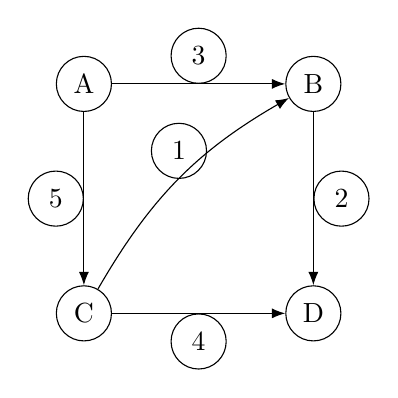
\begin{tikzpicture}[
    >=Latex,
    node distance=22mm,
    every node/.style={circle,draw,minimum size=7mm,inner sep=0pt},
    every edge/.style={draw,->,line width=0.4pt}
  ]
    \node (A) {A};
    \node (B) [right=of A] {B};
    \node (C) [below=of A] {C};
    \node (D) [right=of C] {D};

    \path (A) edge node[above] {$3$} (B)
          (A) edge node[left]  {$5$} (C)
          (B) edge node[right] {$2$} (D)
          (C) edge node[below] {$4$} (D)
          (C) edge[bend left=15] node[above] {$1$} (B);
  \end{tikzpicture}
  \caption{网络图示例}
  \label{fig:graph_example}
\end{figure}


若边上附带距离、时间、能耗、风险等代价信息，则称该图为带权图；反之，若边仅表示连接关系而不包含额外代价，则称为无权图.由于本文讨论的最短路径问题本质上是以路径代价最小化为目标，因此后文默认研究对象均为带权图.

\subsection{图的存储格式}

图的存储方式会直接影响后续算法的访问效率与空间开销.若采用邻接矩阵进行存储，对于含有 $n$ 个顶点的图，需要 $O(n^2)$ 的存储空间.当图较为稀疏，即满足 $m\ll n^2$ 时，邻接矩阵中将包含大量无效元素，从而造成明显的空间浪费.

因此，在实际工程实现中，更常采用适用于稀疏图的邻接表及其压缩存储形式.本文主要涉及两类常见的稀疏存储结构，即 COO（Coordinate）格式与 CSR（Compressed Sparse Row）格式.

其中，COO 格式使用三个长度为 $m$ 的一维数组分别记录每条边的起点索引、终点索引以及对应权值.该格式结构直观、实现简单，适合用于图结构的构造与调试.

与之相比，CSR 格式在 COO 的基础上进一步压缩了行索引信息.它通常使用 \texttt{row\_ptr}、\texttt{col\_indices} 和 \texttt{value} 三个数组来描述图结构，其中 \texttt{row\_ptr[i]} 与 \texttt{row\_ptr[i+1]} 共同确定了第 $i$ 个顶点所有出边在 \texttt{col\_indices} 与 \texttt{value} 中对应的存储区间.相比 COO，CSR 在按顶点批量访问邻接边时更加高效，同时能够在保证结构信息完整的前提下进一步节省空间.图~\ref{fig:csr_storage} 展示了邻接矩阵 $C$ 与 CSR 存储格式之间的对应关系.可以看出，CSR 并未改变图原有的拓扑结构，而只是对其进行了更紧凑的线性化表达.由于本文后续涉及线图构建、邻接展开以及 GPU 并行访存等操作，CSR 形式也更符合后续算法实现的需求.

\begin{figure}[H]
  \centering
  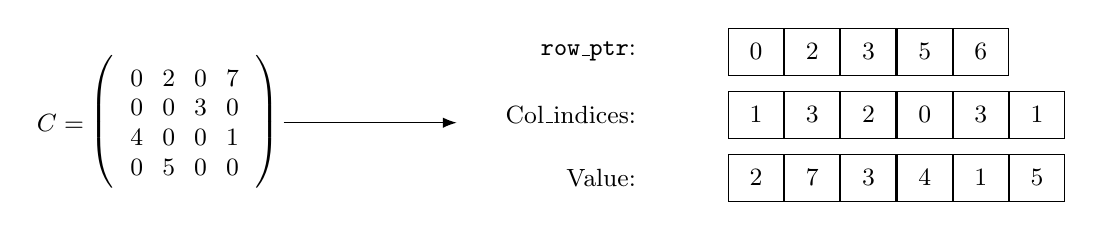
\begin{tikzpicture}[
    >=Latex,
    font=\small,
    box/.style={draw,minimum height=6mm,minimum width=7mm,inner sep=1.5pt},
    label/.style={anchor=east},
    arr/.style={->,line width=0.45pt}
  ]
    % Left: adjacency matrix C
    \matrix (C) [matrix of math nodes, left delimiter={(}, right delimiter={)},
      nodes={inner sep=1.2pt}, row sep=2.5pt, column sep=4.5pt] {
      0 & 2 & 0 & 7 \\
      0 & 0 & 3 & 0 \\
      4 & 0 & 0 & 1 \\
      0 & 5 & 0 & 0 \\
    };
    \node[left=3mm of C.west] {$C=$};

    % Anchor for CSR block (shift right to avoid overlaps)
    \coordinate (csr) at ([xshift=50mm]C.east);
    \draw[arr] ([xshift=4mm]C.east) -- ([xshift=26mm]C.east);

    % Right: CSR arrays
    \node[label] (rpl) at ([yshift=9mm]csr) {\texttt{row\_ptr}:};
    \node[box] (rp0) at ([xshift=14mm,yshift=9mm]csr) {0};
    \node[box] (rp1) [right=0pt of rp0] {2};
    \node[box] (rp2) [right=0pt of rp1] {3};
    \node[box] (rp3) [right=0pt of rp2] {5};
    \node[box] (rp4) [right=0pt of rp3] {6};

    \node[label] (cil) at ([yshift=1mm]csr) {Col\_indices:};
    \node[box] (ci0) at ([xshift=14mm,yshift=1mm]csr) {1};
    \node[box] (ci1) [right=0pt of ci0] {3};
    \node[box] (ci2) [right=0pt of ci1] {2};
    \node[box] (ci3) [right=0pt of ci2] {0};
    \node[box] (ci4) [right=0pt of ci3] {3};
    \node[box] (ci5) [right=0pt of ci4] {1};

    \node[label] (val) at ([yshift=-7mm]csr) {Value:};
    \node[box] (v0) at ([xshift=14mm,yshift=-7mm]csr) {2};
    \node[box] (v1) [right=0pt of v0] {7};
    \node[box] (v2) [right=0pt of v1] {3};
    \node[box] (v3) [right=0pt of v2] {4};
    \node[box] (v4) [right=0pt of v3] {1};
    \node[box] (v5) [right=0pt of v4] {5};
  \end{tikzpicture}
  \caption{CSR 格式存储示意图}
  \label{fig:csr_storage}
\end{figure}

\section{最短路径问题}


\subsection{单源最短路径问题的定义}

\begin{definition}
在图 $G(V, E, W)$ 中，若边集合 $(v_i, v_{i+1}), (v_{i+1}, v_{i+2}), \ldots, (v_{p-1}, v_j)$ 存在，则序列 $p = \langle v_i, v_{i+1}, \ldots, v_j \rangle$ 称为从点 $v_i$ 到点 $v_j$ 的一条路径.为方便表述复杂网络中的边，图的单条边也常由希腊字母 $\alpha, \beta$ 等直接表示.路径 $p$ 的距离（或代价值）定义为
\[
f(p) = \sum_{k=i}^{j-1} w(v_k, v_{k+1}).
\]
\end{definition}

\begin{definition}
最短路径是指从起点 $s$ 到点 $v_j$ 的所有路径中，使得路径长度（即所有边权重之和）最小的路径.若存在多条最短路径，则任选其一作为最短路径.最短路径长度为
\[
d(v_i, v_j) = \min(f(p)),
\]
其中 $p$ 为所有从 $v_i$ 到 $v_j$ 的路径集合中的任意路径.
\end{definition}

\begin{definition}
设 $u$ 和 $v$ 是图 $G(V, E, W)$ 中两个顶点，$w(u,v)$ 表示顶点 $u$ 到点 $v$ 的边的权重，$d(u)$ 和 $d(v)$ 分别表示源点 $s$ 到顶点 $u$ 和顶点 $v$ 的最短距离.如果 $d(u) + w(u,v) < d(v)$，则更新 $d(v)$ 为 $d(u) + w(u,v)$.这一过程就是松弛操作.
\end{definition}

单源最短路径问题即求源点到所有顶点的最短路径，核心操作为反复松弛.

\subsection{经典最短路径问题算法}

随着对最短路径问题研究的不断深入，相关领域提出了多种经典求解方法.其中，Dijkstra 算法作为早期最具代表性的经典算法之一，在边权非负的单源最短路径问题中具有重要地位；而 $\Delta$-Stepping 算法则在传统最短路径算法基础上进一步发展而来，兼具较好的求解效率与并行实现潜力.因此，本节将围绕 Dijkstra 算法与 $\Delta$-Stepping 算法展开介绍，并分析其基本思想、实现特点及适用条件.

\subsubsection{Dijkstra 算法}

Dijkstra算法由荷兰计算机科学家E.W. Dijkstra于1956年提出，是解决单源最短路径问题最常用的贪心算法.该算法适用于所有边权重均为非负的有向图或无向图.


算法思想：Dijkstra算法采用贪心策略，每次从未访问的顶点中选择距离源点最近的顶点，将其加入已访问集合，并据此更新其他顶点的最短距离.通过对所有顶点的这样处理，最终可得到从源点到所有其他顶点的最短路径.


时间复杂度：采用二叉堆实现的Dijkstra算法时间复杂度为 $O((|V| + |E|) \log |V|)$；采用线性查找实现的Dijkstra算法时间复杂度为 $O(|V|^2)$.


算法伪代码：

\begin{algorithm}[H]
  \SetAlgoLined
  \caption{Dijkstra Algorithm}
  \label{algo:dijkstra}
  
  Input: Graph $G = (V, E, W)$, source vertex $s$\\
  Output: Shortest distances $d(v)$ for all $v \in V$\\
  
  Initialization:\\
  \For{each $v \in V$}{
    $d(v) \leftarrow \infty$\
  }
  $d(s) \leftarrow 0$\
  $T \leftarrow V/s$\
  
  \While{$T$ is not empty}{
    Min: $u \leftarrow \{v : v \in T \text{ and } \forall c \in T, d(v) \leq d(c)\}$\
    
    \If{$d(u) = \infty$}{
      break\
    }
    
    Remove $u$ from $T$\
    
    Relax:\
    \For{each $(u, v) \in E$}{
      \If{$d(u) + w(u, v) < d(v)$}{
        $d(v) \leftarrow d(u) + w(u, v)$\
      }
    }
  }
  
  \Return{$d$}\
\end{algorithm}

在上述伪代码中，$d(v)$ 表示源点 $s$ 到顶点 $v$ 的最短距离，$T$ 表示未处理顶点的集合，$w(u, v)$ 表示边 $(u, v)$ 的权重.

算法步骤说明：
\begin{enumerate}
  \item 初始化：将所有顶点的距离初始化为无穷大，源点距离为0，未处理顶点集合 $T$ 为除源点外的所有顶点.
  \item 主循环：当存在未处理的顶点时，重复以下步骤：
  \begin{enumerate}
    \item 从未处理顶点集合 $T$ 中选择距离最小的顶点 $u$.
    \item 若 $d(u) = \infty$，说明剩余顶点不可达，退出循环.
    \item 将顶点 $u$ 从集合 $T$ 中移除.
    \item 对从 $u$ 出发的所有边执行松弛操作，若发现更短路径则更新距离.
  \end{enumerate}
  \item 输出：返回所有顶点的最短距离数组 $d$.
\end{enumerate}

优缺点分析：
\begin{itemize}
  \item 优点：计算效率高，时间复杂度为 $O((|V|+|E|)\log|V|)$（使用优先队列实现）；适用于边权非负的单源最短路径问题.
  \item 缺点：无法处理带有负权边的图；对于稠密图，优先队列的操作可能导致性能下降.
  \item 与非加性问题的联系：Dijkstra算法依赖于边权的加性性质，无法直接应用于非加性问题，需要对问题进行转化或设计新的算法.
\end{itemize}

\subsubsection{\texorpdfstring{$\Delta$}{Delta}-Stepping 算法}

为了解决 Dijkstra 算法中严格的优先队列带来的难以并行化问题，Meyer 等人于 2003 年提出了 $\Delta$-Stepping 算法.该算法通过引入“桶（Bucket）”数据结构，在 Dijkstra 算法与 Bellman-Ford 算法之间取得了良好的平衡，从而实现了对图数据结构的有效并行处理.

\textbf{算法思想}：$\Delta$-Stepping 算法的核心在于将优先队列离散化为一系列连续的桶数组 $B$.设定一个步长参量 $\Delta > 0$，每个桶 $B_i$ 用于存放当前暂定距离 $d(v)$ 落在区间 $[i\Delta, (i+1)\Delta)$ 范围内的顶点.在每一轮迭代中，算法并发地从当前非空的编号最小的桶中取出所有顶点，并使用它们的临接“轻边”（权重 $\le \Delta$ 的边）去更新其后继顶点的距离.如果更新后的顶点距离落入了更小的桶区间，则将其移入对应的桶中.当当前桶内的顶点经过轻边完全松弛稳定后，再利用与之相连的“重边”（权重 $> \Delta$ 的边）进行一轮跨桶范围的并行扩展松弛.

\textbf{时间复杂度}：对于带最大度数限制的随机图拓扑结构，利用并行模型实现的 $\Delta$-Stepping 算法其平均时间复杂度可趋近于 $O(|V| + |E| + \frac{L}{\Delta})$，其中 $L$ 为最长最短路径距离.

\textbf{在非加性并行寻路中的应用机理}：在应对如线图高阶网格这种极度稠密网络且由于需要处理千万级节点状态的背景下，$\Delta$-Stepping 算法有效地避免了并行线程对于单一队列的锁争用（Lock Contention）.通过控制共享变量的并发原子访问（如使用 \texttt{atomicMin}），本算法可以在现代 GPU 计算管线上直接映射为无强制排序的桶内波前探索操作，这也是其在海量数据非加性路由重构系统内进行寻优加速的直接理论基础.

\section{非加性最短路径问题}

非加性最短路径问题放宽了加性假设，使边权可能随上下文、时间或约束变化，导致经典算法失效.本节说明定义、失效原因、现实普适性，并据此给出分类与求解思路.

\subsection{定义与性质}

最短路径的核心是路径成本函数.若路径成本可写成各边固定权重的算术和，则属于加性最短路径；否则即为非加性最短路径.

\subsubsection{加性最短路径问题的定义}

\begin{definition}[加性最短路径问题]
设路径 $p = \langle v_0, v_1, v_2, \ldots, v_k \rangle$ 为从源点 $v_0 = s$ 到终点 $v_k = t$ 的路径，若路径的总成本满足
\[
    f(p) = \sum_{i=0}^{k-1} w(v_i, v_{i+1}),
\]
即“等于路径所经过各边权重的算术和”，且“各边的权重为恒定的、与路径中其他边无关的固定值”，则称该最短路径问题为加性最短路径问题（Additive Shortest Path Problem, ASPP）.
\end{definition}

加性问题的核心特征包括：

（1）边权的独立性和恒定性：在加性最短路径问题中，每条边 $(u, v)$ 的权重 $w(u, v)$ 是预定义的、恒定的常数，与该边在路径中的位置、路径中的其他边、或任何其他上下文无关.这是加性问题最本质的假设，保证了成本的可预测性与确定性.

（2）无后效性（Memoryless Property）：子路径的成本独立于路径的后续扩展，即对任意路径 $p_1 = \langle s, \ldots, u \rangle$ 和 $p_2 = \langle u, \ldots, t \rangle$，有
\[
    f(p_1 \oplus p_2) = f(p_1) + f(p_2),
\]
其中 $\oplus$ 表示路径拼接.历史信息（前面的路径）对未来成本无影响.

（3）最优子结构（Optimal Substructure）：最优路径必然由各段局部最优子路径构成.若 $p^* = \langle s, \ldots, u, \ldots, t \rangle$ 是从 $s$ 到 $t$ 的最优路径，则 $p^*$ 中从 $s$ 到 $u$ 的子路径必为 $s$ 到 $u$ 的最优路径.这直接导出递推关系
\[
    d(t) = \min\{d(u) + w(u, t) : (u, t) \in E\},
\]
这是 Dijkstra、Bellman-Ford 等经典贪心与动态规划算法高效求解的理论根基.

\subsubsection{非加性最短路径问题的定义}

\begin{definition}[非加性最短路径问题]
若路径总成本 $f(p)$ 不能表示为
\[
  f(p) = \sum_{i=0}^{k-1} w(v_i, v_{i+1}),
\]
或边权不再恒定、独立（随时间、位置或历史决策变化），则该最短路径问题称为非加性最短路径问题（Non-additive Shortest Path Problem, NASPP）.
\end{definition}

非加性问题破坏了加性假设的至少一条，带来三类失效：

边权动态性与耦合性：权重依赖时间、路径位置或先前选择，如时变网络 $w(u,v,t)$、容量受限网络的拥塞反馈、多目标场景的向量权重 $\mathbf{w}(u,v)$.

无后效性失效：历史决策影响后续成本，例如车辆疲劳模型、带宽占用导致后续代价（如转弯代价等）依赖当前及前驱路径 $\alpha, \beta$.

最优子结构破坏：全局最优不能由子问题最优递推，如极值型目标 $f(p)=\max w(v_i,v_{i+1})$、多目标 Pareto 优化、带全局约束的可行性组合.

\subsection{问题分类}

非加性最短路径问题在实际应用中具有广泛来源，其表现形式也较为多样.与传统加性最短路径问题相比，这类问题的共同特点在于：路径总代价不再单纯由各边固定权重的线性累加所决定，而往往会受到约束条件、环境状态、路径历史或多属性耦合关系的影响.为了便于后文针对不同问题特征选择相应的建模与求解方法，本节对较为常见的几类非加性最短路径问题进行归纳和说明.需要指出的是，本文后续重点讨论的是路径依赖型非加性最短路径问题，因此其余几类问题主要作为背景性分类进行概述，不作深入展开.

\subsubsection{瓶颈路径问题}

瓶颈路径问题（Bottleneck Path Problem）并不以路径总代价最小作为优化目标，而是关注路径上的“最薄弱环节”或“关键限制因素”.其典型形式包括最小化路径上的最大边权，即 min-max 问题；以及最大化路径上的最小边权，即 max-min 问题，后者也常被称为最宽路径问题.这类模型通常用于描述带宽路由、运输载重限制、桥梁限高、最大风险暴露控制等应用场景.在这些问题中，决定路径优劣的往往不是各段代价的总和，而是其中最不利的一段边或最受限制的一类资源，因此其目标函数本质上不满足经典最短路径中的线性可加结构.尽管如此，由于瓶颈目标具有较强的结构特征，在某些特定情形下仍可借助生成树、阈值判定或改造后的贪心方法实现多项式时间求解.从分类角度看，这类问题说明：一旦路径评价标准由“总和最优”转变为“极值最优”，最短路径问题便已偏离传统加性框架\cite{pollack1960maxcap,edmonds1972theoretical,camerini1984random,gj1979np}.

\subsubsection{资源约束型最短路径问题}

资源约束型最短路径问题（Resource Constrained Shortest Path Problem, RCSP）是在路径成本最优化的基础上，进一步引入时间窗、电量、容量、预算、服务时限等附加资源约束的一类问题.在这类问题中，路径是否可行不仅取决于当前所处节点，还取决于此前路径上已经消耗了多少资源，因此路径的可行性与历史累计状态之间存在紧密联系.也就是说，即便两条路径到达同一节点，只要它们在资源使用情况上不同，后续可扩展性也可能完全不同.这种特征决定了问题求解过程中通常需要同时维护“成本 + 资源状态”的复合信息，而不能仅用单一距离值描述节点状态.随着资源维度的增加，状态空间往往迅速膨胀，导致问题复杂度显著提升，因此该类问题在一般形式下通常属于 NP-hard.实际求解中，常见方法包括标签算法、动态规划剪枝、列生成以及整数规划等.资源约束型问题表明，非加性的一个重要来源，是“路径的历史消耗”对后续决策空间的持续影响\cite{pugliese2013survey,irnich2005spprc,barnhart1998branch,bode2012cutfirst}.

\subsubsection{多属性非线性组合最短路径问题}

多属性非线性组合最短路径问题是指路径优劣不再由单一指标决定，而是需要同时综合时间、费用、风险、能耗、舒适性等多个属性进行评价.在许多现实应用中，这些属性之间并不是简单的线性加权关系，而常常通过某种非线性效用函数、风险函数或偏好函数进行组合.例如，用户对“更快但更贵”与“更便宜但更慢”的选择偏好，往往不能仅通过固定线性权重准确刻画；又如，当风险随累计暴露时间非线性增加时，路径总代价也不再是边权的简单叠加.在这种情况下，问题的目标函数通常不具备经典最短路径所要求的可分解性和最优子结构，因而难以直接应用 Dijkstra 等传统算法.该类问题通常需要结合多目标优化、鲁棒优化、效用建模或 Pareto 最优分析等方法进行处理.从本质上看，这类问题强调的是“多维属性之间的非线性交互”如何打破路径代价的线性累加机制\cite{ehrgott2005multicriteria,deb2002nsga2,kim2006adaptive,bertsimas2004price}.

\subsubsection{时间依赖型最短路径问题}

时间依赖型最短路径问题（Time-Dependent Shortest Path Problem, TDSP）是指边权会随出发时刻或到达时刻变化的一类路径优化问题.典型例子包括城市交通网络中的拥堵变化、公共交通系统中的发车时刻表、机场航班衔接网络以及物流调度中的动态通行时间等.在这类问题中，同一条边在不同时间通过时可能具有完全不同的代价，因此边权不再是静态常数，而是一个与时间状态相关的函数.这样一来，路径总代价不仅依赖于所选边集本身，还依赖于路径经过这些边时所对应的具体时刻.由于“到达当前边的时间”本身又由此前路径决定，因此路径成本会表现出明显的动态耦合特征.时间依赖型问题的难点在于，路径的局部选择会改变后续边的实际代价，从而使得传统最短路径中的静态边权假设失效.对于此类问题，研究中常借助时间扩展图、时间标签更新以及满足 FIFO 条件下的动态最短路径算法进行建模和求解\cite{cooke1966shortest,orda1990shortest,dean2005fifo,chabini1998discrete}.

\subsubsection{随机性与相关性最短路径问题}

在一些更复杂的实际网络中，边权并不是确定的固定值，而可能表现为随机变量，并且不同边之间还可能存在相关结构.由此产生的随机性与相关性最短路径问题（Stochastic and Correlated Shortest Path Problem, SCSP）通常用于描述具有不确定性的交通网络、通信网络或供应链系统.例如，道路旅行时间可能受到天气、事故和整体交通流状态影响，从而在不同路段之间呈现相关波动；又如，某些网络中的链路失效概率也可能并非相互独立.在这类问题中，路径优化目标可能是最小期望时间、最大到达可靠性、最小方差风险，或者在给定置信水平下最小化某种风险度量.由于需要同时处理概率分布、随机波动以及边间相关性，路径代价的表达方式显然已不满足简单的确定性加法结构.相应地，这类问题在建模和求解上通常需要引入随机规划、鲁棒优化、采样近似或风险约束等方法.该类问题说明，非加性不仅可能来源于路径历史，也可能来源于环境不确定性及边权之间的统计依赖关系\cite{frank1969probabilistic,nikolova2006approx,birge2011stochastic,bertsimas2011robust}.

\subsubsection{路径依赖型最短路径问题}

路径依赖型最短路径问题是本文重点关注的一类非加性最短路径问题.其核心特征在于，当前一步的代价不仅由当前边本身决定，还会受到此前路径状态的影响，例如前一条边、已访问节点序列、交通转向状态、模式切换状态，或者累计资源消耗等.换言之，在这类问题中，系统的真实状态已经不再只是“当前所在节点”，而应当表示为“当前节点 + 历史状态”的组合.这意味着，即便两条路径到达同一个节点，只要它们的历史不同，后续扩展所产生的代价和可行性也可能不同.正是这种对历史信息的依赖，使得问题的状态空间迅速膨胀，也使得传统基于节点最短距离递推的经典最短路框架难以直接适用.

在路径依赖型问题中，一类最常见、也最具有代表性的情形，是当前转移代价依赖于前一条边，即代价定义在“相邻边对”之上.例如，在道路网络中，车辆从一条边转入下一条边时，可能产生转向惩罚、禁转约束、等待成本或模式切换成本；在这类情况下，代价已经不再属于单条边，而是属于边与边之间的过渡关系.对于这种局部历史依赖问题，线图转换提供了一种较为自然且结构清晰的建模方式：将原图中的边映射为线图中的节点，再将原图中“相邻两条边可以连续连接”的关系映射为线图中的边.经过这一变换，原本依附于相邻边对的代价，可以转化为线图上的静态边权，从而把原问题重新组织为适合标准最短路径框架处理的形式.也正因为如此，本文后续将重点围绕这一路径依赖型问题展开讨论，并进一步分析线图方法在该类问题中的适配性与并行实现潜力\cite{gj1979np,thomas2007timepath,irnich2005spprc,desaulniers2014vrptw}.

\subsection{路径依赖型最短路径问题的经典算法}

在非加性最短路径问题的六大分类中，路径依赖型最短路径问题具有显著的代表性和研究价值.其核心特征是：当前边或转移的成本不仅取决于边本身，还取决于之前经过的路径历史（如已访问节点序列、累计资源消耗、转向惩罚等）.由于路径依赖性的引入，问题状态空间从单一节点扩展为“节点 + 历史路径/状态”的组合，导致状态空间指数级增长，最优子结构性质失效，问题复杂度通常为 NP-hard\cite{gj1979np}.鉴于本文后续研究将聚焦于此类问题，本节重点介绍两类经典求解算法，并分析其局限性，为第三章线图转换方法的引入奠定基础.

\subsubsection{标签算法（Labeling Algorithm）}

标签算法是求解路径依赖型最短路径问题的经典精确方法，其基本思想是为每个节点维护多个标签来表示"到达该节点的不同历史状态"\cite{irnich2005spprc}.为便于描述，设原图 $G=(V,E)$，源点为 $s$，目标点为 $t$.一个标签可抽象为
\[
  \ell = (v,\; g,\; \mathbf{r},\; h),
\]
其中 $v\in V$ 表示当前节点，$g$ 表示累计成本，$\mathbf{r}$ 表示资源消耗（可为多维），$h$ 表示关键历史信息（例如已访问节点集合、上一步边/转向状态等）.标签算法通过扩展标签生成新标签，并利用支配规则进行剪枝：若在同一节点 $v$ 上，标签 $\ell_A$ 在成本与资源等维度上均不劣于 $\ell_B$，且其历史信息不比 $\ell_B$ 更“受限”（从而任意后续扩展都不会更差），则称 $\ell_A$ 支配 $\ell_B$，可安全删除 $\ell_B$.标签算法的伪代码如算法\ref{algo:pdsp_labeling}所示.

\begin{algorithm}[H]
  \SetAlgoLined
  \caption{Labeling Algorithm for Path-Dependent Shortest Path}
  \label{algo:pdsp_labeling}

  Input: Graph $G=(V,E)$, source $s$, target $t$; transition cost $c(u,v,h)$; state update $h'\!=\!\tau(h,u,v)$; feasibility check $\textsc{Feasible}(\mathbf{r}')$\\
  Output: Best label reaching $t$ (and its path)\\

  Initialization:\\
  For each $v\in V$, set label set $\mathcal{L}(v) \leftarrow \emptyset$\\
  Create initial label $\ell_0=(s,0,\mathbf{0},h_0)$ and insert into $\mathcal{L}(s)$\\
  Initialize a queue (or priority queue) $Q\leftarrow\{\ell_0\}$\\

  \While{$Q$ is not empty}{
    Pop a label $\ell=(u,g,\mathbf{r},h)$ from $Q$\\
    \If{$\ell$ is dominated by some label in $\mathcal{L}(u)$}{
      continue\\
    }
    \For{each outgoing edge $(u,v)\in E$}{
      $h' \leftarrow \tau(h,u,v)$\\
      $\mathbf{r}' \leftarrow \textsc{UpdateRes}(\mathbf{r},u,v,h)$\\
      \If{$\textsc{Feasible}(\mathbf{r}')$}{
        $g' \leftarrow g + c(u,v,h)$\\
        Create new label $\ell'=(v,g',\mathbf{r}',h')$\\
        \If{$\ell'$ is not dominated by labels in $\mathcal{L}(v)$}{
          Remove from $\mathcal{L}(v)$ all labels dominated by $\ell'$\\
          Insert $\ell'$ into $\mathcal{L}(v)$ and push $\ell'$ into $Q$\\
        }
      }
    }
  }

  \Return{the best (minimum-$g$) label in $\mathcal{L}(t)$}\\
\end{algorithm}

伪代码说明：
\begin{itemize}
  \item 标签的含义：同一节点 $v$ 上的不同标签对应不同的“到达方式”，它们携带了导致后续代价差异的历史信息 $h$ 与资源状态 $\mathbf{r}$.
  \item 扩展与更新：沿边 $(u,v)$ 扩展时，用 $\tau(\cdot)$ 更新历史状态（例如更新“上一条边/转向方向”或把访问节点加入集合），并用 $\textsc{UpdateRes}$ 更新资源消耗；同时用 $c(u,v,h)$ 计算依赖历史的边代价.
  \item 支配剪枝：在 $\mathcal{L}(v)$ 内做支配判断，保留“潜在更优且更可扩展”的标签，删除明显不可能产生最优解的标签，以减少搜索空间.
\end{itemize}

方法局限性：尽管标签算法可保证在给定支配规则与状态刻画下找到全局最优解，但标签数量往往随路径长度呈指数增长，导致内存消耗巨大；支配判断本身在多维资源与复杂历史编码下代价较高；并且标签扩展具有强数据相关性，整体过程偏串行，难以直接高效并行化，因而在大规模图或实时场景下计算效率受限.

\subsubsection{列生成与分支定价方法（Column Generation / Branch-and-Price）}

除直接在节点上维护多标签外，路径依赖型最短路径问题在运筹优化中还常被放入“列生成（column generation）/分支定价（branch-and-price）”框架中求解.其核心思想是：不显式枚举所有可行路径，而是把“从 $s$ 到 $t$ 的一条可行路径”视为一个变量（列），在主问题中选择若干列使目标最小；随后通过定价子问题按需生成能够改进目标的路径列.

形式上，可将每条可行路径 $p\in\mathcal{P}$ 赋予成本 $C(p)$（其中 $C(\cdot)$ 可依赖历史/资源/状态演化），令二元变量 $x_p\in\{0,1\}$ 表示是否选择路径 $p$.在只选一条 $s$--$t$ 路径的基本情形下，主问题可写为
\[
  \min\ \sum_{p\in\mathcal{P}} C(p)\,x_p,\qquad
  \text{s.t.}\ \sum_{p\in\mathcal{P}} x_p = 1,\ x_p\ge 0\ (\text{或 }x_p\in\{0,1\}).
\]
由于 $|\mathcal{P}|$ 往往极大，列生成从一个小的路径集合 $\mathcal{P}_0$ 开始求解受限主问题（RMP），并根据对偶信息构造“约化成本（reduced cost）”来寻找新的改进列；若考虑整数性，则在分支过程中反复进行列生成，即形成分支定价框架.

\begin{algorithm}[H]
  \SetAlgoLined
  \caption{Column Generation Framework for Path-Dependent Shortest Path}
  \label{algo:pdsp_column_generation}

  Input: Feasible path set $\mathcal{P}$ (implicit), path cost $C(p)$; initial columns $\mathcal{P}_0$\\
  Output: Best path (integral if solved with branching)\\

  Initialization:\\
  Set working columns $\mathcal{P}_R \leftarrow \mathcal{P}_0$\\

  \Repeat{no improving column found}{
    Solve Restricted Master Problem (RMP) over $\mathcal{P}_R$ and get duals $\pi$\\
    Pricing: find a feasible path $p^*\in\mathcal{P}$ minimizing reduced cost $\bar C(p)=C(p)-\pi$\\
    \If{$\bar C(p^*) < 0$}{
      Add $p^*$ into $\mathcal{P}_R$\\
    }
  }

  \If{integrality is required}{
    Apply branching rules and repeat column generation in nodes (branch-and-price)\\
  }

  \Return{best path implied by final solution}\\
\end{algorithm}

伪代码说明：该框架将“求解路径依赖最短路径”转化为“迭代求解一个小规模主问题 + 反复解定价子问题”.其中定价子问题本质上是在路径依赖约束/状态演化下寻找约化成本最小的可行路径，常见做法是复用标签扩展与支配剪枝等机制在隐式状态空间中搜索，从而避免枚举全部路径.

方法局限性：列生成/分支定价可在大规模组合优化中获得较强的求解能力，但其计算代价通常集中在反复求解定价子问题与分支树扩展上；当路径依赖导致可行路径结构高度复杂时，定价问题本身可能很难、且需要大量标签与支配判断；此外主问题与子问题之间存在强耦合迭代，整体流程同样具有明显串行瓶颈.

\subsubsection{算法局限性与线图转换的动机}

总体而言，无论是直接在图上进行标签扩展与支配剪枝，还是采用列生成/分支定价这类“主问题--定价子问题”的迭代框架，核心困难都绕不开两点：其一是路径依赖带来的隐式状态空间膨胀，使得标签数、可行路径数或搜索分支数迅速增长，从而带来巨大的时间与内存压力；其二是扩展、支配判断与迭代求解具有强数据相关性与顺序依赖，导致并行化与工程落地难度较高.

针对上述局限，本文引入线图（Line Graph）转换作为后续的求解思路：线图将原图的边转化为节点，并将“相邻边之间的依赖关系”显式编码为线图节点间的连接关系，从而把部分路径依赖信息结构化地映射到图结构中.相较于在隐式状态空间中维护大量标签或反复求解定价问题，线图转换在规模增长的可控性、结构规则性以及并行实现方面更具潜力.第三章将系统阐述线图转换的理论基础、算法设计与并行优化策略.

\section{线图理论基础}

在路径依赖型最短路径问题（Path-dependent Shortest Path Problem）中，路径的整体代价不仅取决于单条边的独立权重，还与相邻边之间的组合与连接状态密切相关.传统的图拓扑结构以节点为核心，难以直接刻画边与边之间的动态耦合关系.为了将这种隐藏的“边关系”显式化，引入结构转换机制成为一种有效的解决途径.线图（Line Graph）作为一种经典的图转换方法，通过实现图元素角色的对偶转换，已在图论及复杂网络优化领域得到广泛应用\cite{whitney1932congruent,harary1960some,van1965interchange}.本节将系统梳理线图的基本定义、构造范式及其拓扑性质，为后续求解算法的设计提供坚实的理论支撑.

\subsection{线图的定义}

设原图为 $G=(V,E)$，其对应的线图记为 $L(G)=(V',E')$\cite{whitney1932congruent}.线图的基本思想可概括为“化边为点”：原图中的每一条边 $e\in E$，在转换后的线图中对应为一个顶点；而原图中两条能够首尾相接的边，则在线图中对应为一条连接边.

对于有向图而言，上述规则可以进一步具体化\cite{harary1960some}.设原图中存在两条有向边 $e_1=(u,v)$ 与 $e_2=(v,w)$，若 $e_1$ 的终点恰好是 $e_2$ 的起点，则说明这两条边在原图中可以连续经过.于是，在线图 $L(G)$ 中，便在表示 $e_1$ 与 $e_2$ 的两个顶点之间建立一条有向边 $(e_1,e_2)$.

因此，线图的本质并不是简单复制原图，而是将原图中的“边关系”重新组织为线图中的“点关系”.这一转换使得原本需要借助路径上下文才能识别的边间衔接关系，在线图中被直接编码为显式的邻接结构，为后续刻画边间依赖提供了更直接的表示方式.

\subsection{线图的构造过程}

对于任意有向图 $G=(V,E)$，其线图 $L(G)$ 的构造过程通常可概括为以下几个步骤.

首先，遍历原图中的每一条有向边 $e=(u,v)$，并在线图中为其创建一个对应顶点.换言之，线图的顶点集合由原图的边集合诱导而来.

其次，对原图中任意一对边 $e_1=(u,v)$ 与 $e_2=(v,w)$ 进行检查.若二者满足前一条边的终点等于后一条边的起点，则说明它们在原图中能够构成合法的连续转移，此时在线图中加入一条从 $e_1$ 指向 $e_2$ 的有向边.

最后，对所有满足连接条件的边对重复上述操作，即可得到完整的线图拓扑结构.图~\ref{fig:line_graph_example} 展示了这一转换过程的示意：原图 $G^0$ 的边 $(1,2)$ 与 $(2,4)$ 在线图 $G^1=L(G^0)$ 中分别对应为点 $12$ 与 $24$，并由一条有向边连接.通过该变换，原图中“边与边之间的衔接”被展开为线图中“点与点之间的连接”，从而为后续处理边间依赖提供了更直接的表示方式.

\begin{figure}[H]
  \centering
  \begin{tikzpicture}[
    >=Latex,
    main node/.style={circle,draw,minimum size=6.5mm,inner sep=0pt},
    edge label/.style={draw=none,fill=white,inner sep=1pt,font=\footnotesize},
    every edge/.style={draw,->,line width=0.6pt}
  ]
    % Original Graph G
    \begin{scope}[xshift=0cm, yshift=0cm]
      \node[main node] (U)  at (0, 0) {u};
      \node[main node] (X)  at (0, -2.0) {x};
      \node[main node] (V)  at (2.5, -1.0) {v};
      \node[main node] (W1) at (5.0, 0.5) {w$_1$};
      \node[main node] (W2) at (5.0, -2.5) {w$_2$};
      
      \path (U) edge node[edge label, above=2pt, sloped] {$e_1$} (V)
            (X) edge node[edge label, below=2pt, sloped] {$e_4$} (V)
            (V) edge node[edge label, above=2pt, sloped] {$e_2$} (W1)
            (V) edge node[edge label, below=2pt, sloped] {$e_3$} (W2);
            
      \node[draw=none] at (2.5, -3.5) {\textbf{原图:} $G$};
    \end{scope}
    
    % Arrow indicating transformation aligned vertically with the center (-1.0)
    \node[draw=none] (arrow) at (6.6, -1.0) {\huge $\Rightarrow$};
    
    % Line Graph L(G)
    \begin{scope}[xshift=8.5cm, yshift=0cm]
      \node[main node] (E1) at (0, 0) {$e_1$};
      \node[main node] (E4) at (0, -2.0) {$e_4$};
      \node[main node] (E2) at (3.0, 0.5) {$e_2$};
      \node[main node] (E3) at (3.0, -2.5) {$e_3$};
      
      % Shift positions of diagonal labels so they don't visually intersect
      \path (E1) edge node[edge label, above=1pt, sloped] {$(e_1, e_2)$} (E2)
            (E1) edge node[edge label, pos=0.74, above=1pt, sloped] {$(e_1, e_3)$} (E3)
            (E4) edge node[edge label, pos=0.26, above=1pt, sloped] {$(e_4, e_2)$} (E2)
            (E4) edge node[edge label, below=1pt, sloped] {$(e_4, e_3)$} (E3);
      
      \node[draw=none] at (1.5, -3.5) {\textbf{线图:} $L(G)$};
    \end{scope}

  \end{tikzpicture}
  \caption{有向图网络拓扑映射至线图的转换展开结构}
  \label{fig:line_graph_example}
\end{figure}


\subsection{线图的拓扑性质}

线图在拓扑结构层面呈现出若干关键性质，这些性质是后续算法设计的核心依据：

（1）拓扑规模扩张性

线图的节点规模严格等于原图的边规模，即：
$$ |V(L(G))| = |E(G)| $$ 
由于实际网络（如交通网、通信网）通常满足 $|E| \gg |V|$，线图变换会导致图规模的非线性扩张.这一特性提示我们在算法设计时，必须考量由于状态空间膨胀带来的存储与计算开销问题.

（2）邻接语义的重定义

在线图空间中，“邻接关系”不再表征地理或物理节点的直接连通，而是刻画原图中不同路段之间的“时空衔接连贯性”.这使得线图具备了捕获原图高阶路径结构特征的能力.

（3）路径结构的同构映射

原图空间中的任意一条可行路径：
$$ P_G = v_1 \rightarrow v_2 \rightarrow \cdots \rightarrow v_k $$ 
在线图空间中存在唯一对应的一条路径：
$$ P_{L(G)} = (v_1,v_2) \rightarrow (v_2,v_3) \rightarrow \cdots \rightarrow (v_{k-1},v_k) $$ 
这种严格的同构映射不仅保证了路径连通性的无损传递，也确保了在双域间进行最优性检索的等价性.

（4）依赖信息的显式表征优势

由于线图的顶点直接关联原图的边，研究者可在线图顶点或连边上灵活挂载多维属性矩阵.例如，可将转弯延误、路口惩罚或复杂的边际交互成本直接编码为线图的边权.这一性质从根本上消除了经典图结构在处理“非马尔可夫型”路径成本时的表达瓶颈.

\subsection{线图在最短路径求解中的应用机理}

在经典最短路径范式中，路径评价体系通常遵循严格的线性可加性假设.然而，在面对包含复杂转弯限制或状态相依成本的非加性网络时，贝尔曼最优性原理（Bellman's Principle of Optimality）往往失效，导致 Dijkstra 等传统算法难以直接适配.

引入线图理论可实现问题域的降维重构.具体映射机理如下：

\begin{itemize}
  \item 状态转移：将原图难以处理的“边间耦合约束”转化为线图中常规的“节点与边权属性”；
  \item 成本线性化：将非加性的路径依赖成本吸收进线图的拓扑结构中，使得转换后的线图重新满足权值累加原则.
\end{itemize}

经过此类同构变换，复杂的路径依赖型最短路径问题被优雅地还原为线图空间下的标准最短路径问题.此时，不仅传统的高效路由算法能够重新发挥效用，且线图本身高度规则的矩阵特征也为引入现代并行计算框架（如 GPU 加速）创造了有利条件.

值得注意的是，若非加性成本不仅仅取决于前一条边，而是依赖于前 $k$ 条边的路径历史，则此类问题可以通过构造高阶线图（Higher-order Line Graph，记为 $L^{[k]}(G)$）来解决.高阶线图通过迭代转换，将长为 $k$ 的边序列压缩为单个节点，从而能精确结构化表达具有有限阶局部马尔可夫性质（即 $k$-加性）的复杂路径代价.

\section{CUDA并行框架概述}

为了求解由线图经过规模扩张后的非加性最短路径问题，利用图形处理器（GPU）强大的高并发特性成为提升算法效率的关键.CUDA（Compute Unified Device Architecture）是由 NVIDIA 推出的通用并行计算架构，它通过提供一套统一的软硬件计算框架，使得开发者能够使用 C/C++ 等高级语言直接对 GPU 进行编程，从而将传统的串行复杂图计算任务转化为高度并行的软硬件协同计算.
本节将简要介绍与后续算法设计密切相关的 CUDA 软件架构及其硬件编程模型.

\subsection{CUDA 软件架构}

CUDA 的软件架构在逻辑上基于统一和分层的设计理念，向开发者屏蔽了底层 GPU 硬件的复杂性.其核心思想是“异构计算（Heterogeneous Computing）”，即 CPU 与 GPU 协同工作，各司其职：
\begin{itemize}
    \item \textbf{主机（Host）}：通常指代 CPU 及其内存系统.主机端主要负责处理那些复杂的逻辑控制流、串行计算任务以及任务的调度与资源分配.在最短路径求解任务中，主机负责数据预处理（如线图转换）、内存分配及输出结果的回收.
    \item \textbf{设备（Device）}：通常指代 GPU 及其内存（如全局显存等）.设备端被视作一个高度并行的协处理器，接收来自主机端的数据和计算指令.它主要负责执行拥有极高计算密度和高度并行性的任务，例如大规模图结构中数以万计的节点松弛操作及边权重更新.
\end{itemize}
主机程序通过调用 CUDA 提供的运行时 API（Runtime API）或驱动 API（Driver API），向设备端分发名为“核函数（Kernel）”的并行计算代码，进而触发 GPU 的算力释放.

\subsection{GPU 编程模型与内存结构}

在实际的编程模型中，CUDA 将 GPU 计算抽象为多层级的线程组织架构以及层次化存储结构，以适配网络图结构的不同层次访问需求.

\begin{enumerate}
    \item \textbf{线程组织架构}：CUDA 中的最小执行单元是线程（Thread）.在执行一个 Kernel 时，这些线程被组织起来.若干个线程组成一个线程块（Block），线程块内可以通过共享内存和同步屏障机制实现高效协作；多个并行运算的线程块共同集成一个网络（Grid）.对于最短路径图算法，可以把源点集合或者边集合细粒度地分配给每一个线程或线程块并发处理.
    \item \textbf{层次化内存空间}：为了提升数据吞吐量，CUDA 提供多种存储方式：
    \begin{itemize}
        \item \textbf{全局内存（Global Memory）}：容量最大，主从设备皆可访问，常用于存放整个底层的线图拓扑（如邻接表和权重集）和节点的距离数组.
        \item \textbf{共享内存（Shared Memory）}：位于线程块内部，是一种在Block内的低延迟片上存储介质.在执行松弛迭代时，可将局部更新密集的队列或临时变量放入其中缓冲，大幅降低拉取全局内存的访存延迟.
        \item \textbf{寄存器（Registers）}：每个线程所独占的最快缓存，存储线程执行时的私有上下文变量.
    \end{itemize}
\end{enumerate}

通过上述多线程的阵列调度与多层级的访存优化，基于 CUDA 的并行求解能够实现极高的图计算吞吐率.这不仅能有效抵消“线图拓扑扩张”带来的额外性能开销，更从根本上为现代非加性最短路径问题的高效求解提供了强大的物理算力支撑.

\section{本章小结}

本章先回顾了图的基本概念与加性最短路径的经典定义和算法，再形式化给出非加性最短路径问题及其失效机理，归纳现实应用中的普适性与问题类型；随后总结了改写松弛、线图/状态扩展、动态规划及并行近似等求解思路，并介绍了线图转换要点与CUDA并行框架.通过上述讨论不难发现，现实网络中大量存在的路径依赖型惩罚（如交规转弯限制等），在本质上符合局部马尔可夫性质与有限阶加性（$k$-additive）特征.这也意味着，利用线图及其高阶扩展不仅能有效地捕获此类非加性约束并将其转化为标准的静态模型结构，且高度匹配现代GPU并行的计算范式.正是基于这种理论上的天然契合，下一章将以此为切入点，针对具体的 $k$-加性非加性场景进行更深入的框架设计与相应的并行优化.

% !TeX root = ../main.tex

\chapter{线图在非加性最短路径问题中的应用及并行化介绍}


\section{线图转换对非加性问题的适配性分析}

正如第二章所述，现实网络广泛存在如交规转弯惩罚、无人机动态油耗等路径依赖问题，导致传统的加性最短路径前提难以成立。在这些非加性（Non-additive）最短路径问题（或被称为条件权重最短路径问题）中，图网络某条边的通行代价不再是静态常量，而是受到该路径前驱历史状态约束。为了将这类具有局部马尔可夫性质的问题纳入严密的数学框架，近期研究引入了有限图的差分分析（Differential Analysis on Finite Graphs）理论，将任意路径实函数空间定义为 $H(P) = \{f : P \rightarrow \mathbb{R}\}$，并基于特定路径的差分算子 $\partial f(\alpha | p)$ 实现了对各类复杂代价函数的严格分类\cite{durand2024generalized}。

依据该微分形式理论，任何复杂路径的代价都可以被精确拆解为其局部差分的叠加：
\begin{equation}
    f(p) = \sum_{\alpha \in p} \partial f(\alpha | p)
\end{equation}
其中，$P$ 表示图 $G$ 中所有合法路径的集合，$p \in P$ 为某一条具体路径；$\alpha \in E_G$ 表示构成该路径的某一条有向边；算子 $\partial f(\alpha | p)$ 定义为在给定前置历史路径段的情况下，拓展边 $\alpha$ 接入该路径所带来的局部代价增量（即，$\partial f(\alpha|p) = f(p \cup \{\alpha\}) - f(p)$）。

在此基础上，若到达某条目标边 $\alpha$ 的差分代价变动 $\partial f$ 仅受其紧邻的前面 $k$ 条边（即有限深度的历史步骤）的条件影响，则该代价函数在拓扑学上被称为 \textbf{$k$-加性（$k$-additive）函数}，记作 $f \in F^{(k)}_G$。在这一标准下，传统可直接求解的纯加性代价函数被统一归类为 0-加性函数（$F^{(0)}_G$），而大多数涉及转弯角度或前驱关联约束的实际物理模型，均可被抽象降级为条件受限的 1-加性或 2-加性网络路线问题。

针对这种突破了零阶马尔可夫性的 $k$-加性前驱依赖问题，\textbf{线图（Line Graph）转换理论}展现出了良好的结构适配性与算法应用价值：
\begin{itemize}
    \item \textbf{网络状态的降维解耦：} 对于具有 1-加性复杂代价的原图 $G(V_G, E_G)$，其前驱约束使得节点间的状态过渡相互关联。通过将其同态映射为线图 $L(G)$，原图中的有向边映射为线图中的实体节点（即 $V_{L(G)} = E_G$）。这种拓扑转换将原图中附带领航方向的动态历史轨迹转化为线图中静态的独立节点。
    \item \textbf{非加性约束的静态显式加权：} 在原图 $G$ 中，受历史条件所限的转移代价 $\partial f(\beta | \alpha)$（从前驱边 $\alpha$ 跨越节点转移到边 $\beta$ 所产生的额外代价），被等效地合并到了线图 $L(G)$ 中新生成的相邻节点对之间的初始静态边权重中。
\end{itemize}

综上所述，通过线图转换这一空间拓扑工具，我们能够在保留完整物理约束信息的条件下，将源网络上受历史制约的 $k$-加性寻路问题，在数学映射层面等效地重构为替代图 $L(G)$ 上的 0-加性基准问题。这种拓扑变换为全局寻优算法的设计提供了坚实的理论基础。基于此，Durand 等人\cite{durand2024generalized}提出了条件权重最短路径（Conditional Weighting Shortest Path, CWSP）算法框架。下文将首先对该经典算法的具体设计与等价性证明进行详细论述，并为后续提出该算法的并行化改进方案作铺垫。

\section{基于线图的算法设计}

基于前节理论中代价函数的微分分解与拓展思维，现有研究已经建立了一套完整的条件权重最短路径（CWSP）算法框架\cite{durand2024generalized}，用于求解包含复杂前驱约束的最优路径问题。本节将对该框架进行深入剖析，其核心思路分为拓扑转换、条件加权映射与替代图寻路三个层序步骤。

\begin{figure}[H]
    \centering
    \begin{tikzpicture}[
        node distance=1.5cm and 2cm,
        box/.style={rectangle, draw, rounded corners, minimum width=3.5cm, minimum height=1.5cm, align=center, thick, fill=blue!10},
        arrow/.style={-stealth, thick},
        label/.style={font=\small, text width=3cm, align=center}
    ]
        
        % Nodes
        \node[box, fill=gray!10] (input) {原图网络 \\ $G=(V_G,E_G)$ \\ (带前驱物理约束)};
        \node[box, below=of input] (phase1) {第一阶段: 拓扑转换 \\ 节点化连边 \\ $V_H \leftarrow E_G, \, E_H \leftarrow (\alpha,\beta)$};
        \node[box, below=of phase1] (phase2) {第二阶段: 静态加权 \\ 差分增量映射 \\ $W_H \leftarrow \partial f(\beta|\alpha)$};
        \node[box, below=of phase2] (phase3) {第三阶段: 路径寻优 \\ 标准Dijkstra求解 \\ $p^* \leftarrow \min W_H(q)$};
        \node[box, fill=green!10, below=of phase3] (output) {全局最优解 \\ $p^* \in P_G(s,t)$};
        
        % Arrows
        \draw[arrow] (input) -- (phase1);
        \draw[arrow] (phase1) -- (phase2) node[midway, right, label] {无权高阶线图 \\ $L^{[k]}(G)$};
        \draw[arrow] (phase2) -- (phase3) node[midway, right, label] {带权0-加性替代图 \\ $H(V_H,E_H,W_H)$};
        \draw[arrow] (phase3) -- (output);
        
        % Decorative box framing the algorithm phases
        \draw[dashed, thick, gray] 
            ([xshift=-3cm, yshift=0.5cm]phase1.north west) rectangle 
            ([xshift=3.5cm, yshift=-0.5cm]phase3.south east);
        \node[anchor=south west, text=gray, font=\bfseries] at ([xshift=-3cm, yshift=0.5cm]phase1.north west) {CWSP算法核心步骤};
            
    \end{tikzpicture}
    \caption{非加性约束下的线图转换与最短路径求解（CWSP框架）流程}
    \label{fig:cwsp_pipeline}
\end{figure}

\subsection{第一阶段：线图的拓扑替代构造}
算法的第一步旨在将原图 $G=(V_G, E_G)$ 在连边上的隐式约束，物理显式化为图节点的邻接问题。该过程定义了原图到其替代图（Alternative Graph，本质即为线图 $H = L(G)$）的映射逻辑：
\begin{enumerate}
    \item \textbf{节点生成：} 为原图 $G$ 中的每一条有向边 $\alpha \in E_G$ 在新图 $H$ 中创建一个对应的单一实体节点。即新图节点集由原图边集构成：$V_H = \{ u \mid u = \alpha \in E_G \}$。
    \item \textbf{连边构建：} 若在原图 $G$ 中边缘 $\alpha$ 和有向边 $\beta$ 能够顺畅过渡（即边 $\alpha$ 的终点与边 $\beta$ 的起点为同一节点），则在线图 $H$ 中创建一条连接前驱节点与后续节点的新边，即 $E_H = \{ (\alpha, \beta) \mid \alpha, \beta \in V_H, \text{且~} \alpha_2 = \beta_1 \}$。
\end{enumerate}

综上拓扑映射规则，该阶段具体的构造过程如算法 \ref{alg:line_graph} 所示。

\begin{algorithm}[H]
\caption{线图的拓扑替代构造}\label{alg:line_graph}
\KwIn{原图 $G = (V_G, E_G)$}
\KwOut{线图 $L(G)$}
$V_{L(G)} \leftarrow \{(\alpha) \mid \alpha \in E_G\}$\;
$E_{L(G)} \leftarrow \emptyset$\;
\ForEach{$\alpha \in E_G$}{
    \ForEach{$\beta \in E_G$}{
        \If{$\alpha_2 = \beta_1$}{
            $E_{L(G)} \leftarrow E_{L(G)} \cup \{(\alpha, \beta)\}$\;
        }
    }
}
$L(G) \leftarrow (V_{L(G)}, E_{L(G)})$\;
\Return $L(G)$\;
\end{algorithm}

如算法 \ref{alg:line_graph} 所示，该生成过程的核心依赖于遍历原图的边集合 $E_G$。第 4-5 行完成了替代图 $L(G)$ 的节点集和边集的初始化。第 6-12 行通过双层循环枚举所有可能的原图有向边对 $(\alpha, \beta)$，并通过判断前驱边的物理终点 $\alpha_2$ 是否等同于后继边的物理起点 $\beta_1$ 来决定是否在替代图中建立新的有向连接。这种基于有向边前后继关系的重组，构成了替代图 $H$ 的整体拓扑骨架。

\subsection{第二阶段：非加性约束的静态加权}
替代图 $H$ 生成后，需要将蕴含历史约束的非加性网络代价内化到替代图的全新边集合 $E_H$ 中。假定特定问题的非加性网络最多取决于 $k$ 级历史状态，对于生成的替代图上的每条转移连边 $(\alpha, \beta)$，运用公式（3.1）中引入的偏导数评价算子即可算出其固化的静态网络权重：
\begin{equation}
    W_H(\alpha \to \beta) = \partial f(\beta \mid \alpha)
\end{equation}
此时，无论原图问题具有何种形式的约束，都已经通过局部差分值转化为替代图 $H$ 中恒定且静态的网络权重。至此，含有条件约束的复杂网络，已被等效转化为标准权重的纯加性有向图。这一阶段权重映射的整体逻辑如算法 \ref{alg:conditional_weight} 所示。

\begin{algorithm}[H]
\caption{替代图（线图）的条件加权}\label{alg:conditional_weight}
\KwIn{原图 $G = (V_G, E_G)$，复杂代价函数 $f$，代价函数的加性阶数 $k$}
\KwOut{带权替代图 $H = (V_H, E_H, W_H)$，其中 $H$ 本质为高阶线图 $L^{[k]}(G)$}
$H \leftarrow L^{[k]}(G) $ \tcc*{利用算法 \ref{alg:line_graph} 构造高阶线图}
\ForEach{$(u_H, v_H) \in E_H$}{
    $(u_1, \dots, u_{k+1}) \leftarrow u_H$\tcc*{其中 $l(u_H)=l(v_H)=k+1$}
    $(v_1, \dots, v_{k+1}) \leftarrow v_H$\;
    $\beta \leftarrow (u_{k+1}, v_{k+1})$ \tcc*{提取最新扩展边 $\beta \in E_G$}
    $w_{(u_H, v_H)} \leftarrow \partial f(\beta \mid u_H)$ \tcc*{计算差分并赋静态权重}
}
$V_H \leftarrow V_H \cup V_G$\;
\ForEach{$u_H \in V_H$}{
    $u \leftarrow (u_H)_1$\;
    $\gamma \leftarrow (u, u_H)$ \tcc*{从原图节点进入替代图 $H$ 的连边}
    $E_H \leftarrow E_H \cup \{\gamma\}$\;
    $w_\gamma \leftarrow f((u_H)_1, \dots, (u_H)_k)$\;
}
$W_H \leftarrow \{w_e \mid e \in E_H\}$\;
\Return $H = (V_H, E_H, W_H)$\;
\end{algorithm}

算法 \ref{alg:conditional_weight} 详细展示了将动态非加性代价固化为静态权重的计算过程。算法第 1 行首先调用前述逻辑构造高阶替代线图结构。第 2-6 行依次对替代图中的每一条新生成连边 $(p, q)$ 进行遍历，捕捉发生状态过渡的最新连边 $\beta$，随后应用偏导数算子 $\partial f$ 求取对应的局部差分代价，以此作为该条连边的固有静态权重。此外，算法在第 8-13 行针对由原网络起起始点寻路并过渡到替代图的“入界连接边”，单独计算了其初始状态下的边界代价，以此保证算法寻优在总体尺度上的严格数学对齐。

\subsection{第三阶段：基于等效替代图的路径寻优}
完成图结构的拓扑替代及权重重分配后，替代图 $H$ 已转化为标准的 0-加性有向图，此时可直接接入经典的 Dijkstra 算法在此新网络上进行全局寻优。由于模型物理意义的改变，应用 Dijkstra 算法时只需对其停止条件进行相应的逻辑更新。

在原始最短路径问题中，寻路过程当目标节点 $t \in V_G$ 被从优先队列弹出时即告结束。但在替代图 $H$ 结构下，节点实质为原图空间中的一条“转移线段”。因此，Dijkstra 算法的停止条件转变为：当优先队列弹出的当前节点（即某条有向边）的终点，恰好指向原问题的全局目标节点 $t$ 时，寻路探索即告完成。随后，运用回溯法依据前驱指针（predecessor）即可输出映射回原图的完整最小代价通路 $p^*$。针对转换后图结构的单源最短路寻优完整步骤如算法 \ref{alg:dijkstra_sub} 所示。

\begin{algorithm}[H]
\caption{基于替代图（线图）的 Dijkstra 寻路算法}\label{alg:dijkstra_sub}
\KwIn{带权替代图 $H = (V_H, E_H, W_H)$，起点 $s$，终点 $t$}
\KwOut{最优路径 $p^*$}
\ForEach{$v_H \in V_H$}{
    $\text{cost}[v_H] \leftarrow \infty$\;
    $\text{predecessor}[v_H] \leftarrow \emptyset$\;
}
\tcc{此处省略了与起点相关的初始化细节，默认包含从起点关联起步的过程}
$\text{cost}[s'] \leftarrow 0$ \tcc*{$s'$表征线图层级下对应源节点的特定起始状态}
$Q \leftarrow V_H$\;
\While{$Q \neq \emptyset$}{
    $u_H \leftarrow \text{extract-min}(Q)$\;
    \ForEach{连边 $\alpha_H = (u_H, v_H) \in E_H$}{
        \If{$\text{cost}[v_H] > \text{cost}[u_H] + w_{\alpha_H}$}{
            $\text{cost}[v_H] \leftarrow \text{cost}[u_H] + w_{\alpha_H}$\;
            $\text{predecessor}[v_H] \leftarrow u_H$\;
        }
        \If{$(v_H)_{k+1} = t$}{
            $u_{\text{last}} \leftarrow v_H$\;
            \textbf{break}\;
        }
    }
}
$p^* \leftarrow (t)$\;
$u_H \leftarrow u_{\text{last}}$\;
\While{$l(u_H) = k+1$}{
    $v_H \leftarrow u_H$\;
    $u_H \leftarrow \text{predecessor}[v_H]$\;
    $p^* \leftarrow ((u_H)_{k+1}, p^*)$\;
}
$p^* \leftarrow ((v_H)_1, \dots, (v_H)_k, p^*)$\;
\Return $p^*$\;
\end{algorithm}

结合算法 \ref{alg:dijkstra_sub} 可知，在寻路探索阶段的前 14 行，操作逻辑与标准 Dijkstra 算法保持高度一致。主要变化出现在第 15 行为目标节点的核验机制：由于替代图 $H$ 中遍历的节点本质已升级为原图的行进边集，故寻路停止标志更新为针对当前搜寻前沿的终点状态 $v_{k+1}$ 执行判定。一旦该终点触及全局目标节点 $t$，循环即可中止。并在算法第 20-25 行，通过向后递推追踪前驱指针，将替代图域中的节点迹线反向解耦拼装，最终呈现并返回实际地理平面上的单源最优路径。

\subsection{算法理论最优性的论证}
为进一步巩固上述算法设计的理论正确性，现对该 CWSP 算法所求得的最短路径等价于原图 $G$ 非加性问题的最优解，作如下严密证明：

\textbf{定理 3.1（最优性等价定理）} \textit{设给定有向图 $G(V_G,E_G)$ 及由源点 $s$ 至终点 $t$ 的 $1$-加性路径寻优问题，目标函数为 $\min_{p \in P_G(s,t)} f(p)$。设 $H(V_H,E_H,W_H)$ 为依据上述 CWSP 算法第一、二阶段条件加权构造出的线图，则在该图中依据第三阶段求得的纯加性最短路径解集 $\arg\min_{q \in P_H} \sum_{e \in q} W_H(e)$，其必然映射回 $P_G(s,t)$ 并对应 $f(p)$ 的全局最优解。}

\textbf{证明:}

\textbf{步骤一：解空间的双射映射性质（Bijective Mapping of Solution Space）}  
设 $p^* \in P_G(s,t)$ 为原图中的一条有效路径边序列，记为 $p^* = \langle \alpha_1, \alpha_2, \dots, \alpha_n \rangle$，起点判定条件为 $(\alpha_1)_1 = s$，终点为 $(\alpha_n)_2 = t$。依据 CWSP 第一阶段生成规则 $V_H = E_G$ 且 $E_H = \{ (\alpha_i, \alpha_{i+1}) \}$，该序列 $p^*$ 的邻接特征在 $H$ 中唯一显化为一条有效节点路径 $q = \langle v_1, v_2, \dots, v_n \rangle \in P_H$，满足 $v_i = \alpha_i \in V_H$。这也论证了 $P_G$ 与 $P_H$ 解空间之间存在严格的一一双向映射算子 $\Phi : p^* \mapsto q$。

\textbf{步骤二：非加性向加性的代价等价性（Cost Equivalence）}  
基于代价函数的差分分解定义与 $1$-加性截断边界属性，原图中路径 $p^*$ 的组合代价可递推展开：
\begin{align}
    f(p^*) &= f(\langle \alpha_1, \alpha_2, \dots, \alpha_n \rangle) \notag \\
           &= f(\alpha_1) + \sum_{i=1}^{n-1} \partial f(\alpha_{i+1} \mid \langle \alpha_1, \dots, \alpha_i \rangle) \notag \\
           &= f(\alpha_1) + \sum_{i=1}^{n-1} \partial f(\alpha_{i+1} \mid \alpha_i)
\end{align}
而对应由 CWSP 第二阶段权值定义的映射线图路径 $q$ ，其 $0$-加性累积模型为：
\begin{equation}
    W_H(q) = w_{enter}(\alpha_1) + \sum_{i=1}^{n-1} W_H(v_i, v_{i+1})
\end{equation}
定义起始惩罚 $w_{enter}(\alpha_1) = f(\alpha_1)$ 及连边静态权值项 $W_H(v_i, v_{i+1}) = \partial f(\alpha_{i+1} \mid \alpha_i)$ 后，上述两式可建立如下等价关系：$\forall p^* \in P_G(s,t), \, f(p^*) \equiv W_H(\Phi(p^*))$。

\textbf{步骤三：最优解一致性（Optimality Convergence）}  
设经由 CWSP 第三阶段寻路，在 $H$ 平面上求得 $\min_{q \in P_H} W_H(q)$ 对应的最短线路 $q^*$。假定在原图 $G$ 中存在一条总代价更小的有效路径 $p'$ 满足 $f(p') < f(\Phi^{-1}(q^*))$；由于定理证明的映射等价性 $f(p^*) \equiv W_H(q^*)$ 约束，必然在线图 $H$ 中也存在一条对应的有效同构轨迹 $q' = \Phi(p')$，满足 $W_H(q') < W_H(q^*)$。这与“$q^*$ 是 $H$ 中的最小权重路径”这一前提假设相矛盾。
因此，假设不成立，$f(\Phi^{-1}(q^*))$ 必然是全局绝对下确界。这表明了 CWSP 算法解得的 $q^*$ 完全等价于原问题网络的最优解。定理论证闭环，证毕。

需要指出的是，这种在空间维度上扩展网络的 CWSP 算法机制，在线图模型拓展时将面临边数显著增加的情况：即 $|E_{L^m(G)}| \leq n^{m+2}$（$n$为节点数）。这种节点规模的几何级数增长虽然降低了逻辑判断的复杂度，但对传统单线程 CPU 的计算能力带来了特定的挑战。针对这类大规图层遍历与计算需求，引入基于 GPU 底层的 CUDA 高并发阵列进行并行运算，成为了一种有效的解决途径。


\section{算法的并行优化}

针对 CWSP 算法在线图转换及寻路过程中面临的空间规模扩张与计算瓶颈，本节基于 GPU 的 CUDA 并行架构，对算法的三个核心阶段提出针对性的并行化改进方案。主要改进策略包括线图拓扑结构的并行构建、条件权重的并行计算，以及采用适配 GPU 架构的并行最短路径算法替代传统的 Dijkstra 算法。

\begin{figure}[H]
    \centering
    \begin{tikzpicture}[
        node distance=0.8cm and 1cm,
        stepbox/.style={rectangle, draw, rounded corners, minimum width=6cm, minimum height=1.2cm, align=center, thick, fill=orange!10},
        arrow/.style={-stealth, thick},
        font=\small
    ]

    % Draw Grid for GPU
    \draw[thick, draw=green!60!black, rounded corners, loosely dashed] (-4.5, 1.5) rectangle (4.5, -6.5);
    \node[anchor=north west, font=\bfseries\large, text=green!50!black] at (-4.2, 1.2) {GPU (CUDA) 并行架构化};

    % Phase 1: Line Graph Construction
    \node[stepbox] at (0, -0.5) (csr) {第一阶段: 拓扑高并发构建 \\ (CSR度数扫描与前缀和无锁映射)};
    
    % Phase 2: Conditional Weight SIMT
    \node[stepbox] at (0, -3.0) (simt) {第二阶段: 条件权重提取 \\ (SIMT多分支协同与并发访存优化)};
    
    % Phase 3: $\Delta$-Stepping
    \node[stepbox] at (0, .5.5) (delta) {第三阶段: $\Delta$-Stepping寻优 \\ (无序波前松弛与共享内存并发探底)};

    \draw[arrow] (csr) -- (simt);
    \draw[arrow] (simt) -- (delta);

    \end{tikzpicture}
    \caption{基于CUDA架构的线图寻路并行优化策略实施框架}
    \label{fig:parallel_optimization}
\end{figure}

\subsection{线图拓扑结构的并行构建}

在线图生成阶段，原图 $G$ 中每条有向边的拓展及其相邻关系的判定过程相互独立，不存在数据依赖性，这为细粒度的数据并行提供了可能。

在具体并行实现中，必须摒弃传统串行算法中基于动态内存分配的链表或双重循环遍历。为适配 GPU 的内存分层架构，本文采用高聚合的\textbf{压缩稀疏行（Compressed Sparse Row, CSR）}数据格式将原图结构存储于设备全局内存（Global Memory）中，并采用以“边”为粒度的两阶段并行映射策略。

第一阶段为\textbf{拓扑度数扫描与空间预分配}。由于原图中各条边引出的后继边数量（即节点的出度）参差不齐，为了防止各线程在写入连续显存时发生写冲突（Race Condition），首先分配一维的 CUDA 线程网格与线程块。每个线程（Thread）独立读取原图的一条连边 $\alpha$，统计其尾节点对应的合法相连后继边 $\beta_i$ 的数量（即新生成的替代图出度）。随后，调用高效的并行前缀和（Exclusive Prefix Sum / Scan）算法，对所有线程生成的度数数组进行扫描，由此算出替代图总边数并为其预分配连续的稀疏存储空间。同时，该前缀和的结果等同于为每条原图边分配了在全局写入数组中的绝对偏移量（Offset）。

第二阶段为\textbf{无锁化拓扑实例化}。重新启动并行的映射核函数（Kernel），各计算线程根据第一阶段获取的独占偏移量索引，将合法的 $(\alpha, \beta_i)$ 状态转移关系直接、独立地写入 CSR 结构的目标地址中。这种基于前缀和配合 CSR 格式的并行生成模式，实现了完全无锁（Lock-free）的高并发内存加载，极大缩减了大量动态构建替代图拓扑由于互斥锁导致的等待过载。

\subsection{条件权重的并行计算}

线图结构的重构完成后，所有新生成的转移关联边及其对应的原图映射信息已全部存储于连续数组中。此时，为线图赋权的偏导数算子 $\partial f(\beta \mid \alpha)$ 的计算是一个典型的单指令多数据（SIMT）操作。

在这一优化步骤中，直接针对海量新生成的替代图边集合 $E_H$ 启动一维计算核函数。每个执行线程依据其全域线程索引（Global Thread ID），精确映射并提取出一条拓扑转移变 $e_H = (\alpha, \beta)$。随后，线程依据内存中的几何与前趋历史状态属性，并行地对每一过渡关系（如计算转弯角度惩罚、油耗受阻损耗等）进行评价，继而产生代价差分增量并将其固化为静态图权值。

为进一步榨取计算管线性能，此阶段必须引入以下两项底层显存与并发约束策略：首先是\textbf{合并内存访问（Memory Coalescing）}。由于前阶段所建立的替代图连边已由连续的 CSR 格式紧凑存储于主显存，相邻计算线程在提取 $(\alpha, \beta)$ 指针特征时，其内存寻址呈现出高度的空间局部性，能够以宽总线事务的数据块形式并发出队，从硬件层面填满极速的显存带宽吞吐；其次是\textbf{线程束控制冲突抑制（Warp Divergence Control）}。复杂的物理重定权往往依赖“是否合规转弯”、“死路惩罚阈值”等多分支的 \texttt{if-else} 逻辑评判。此并行设计借由条件算子与内部谓词判定（Predication）等形式有效替换显式的控制流拆分，借以保证指派往同一线程束（Warp，即在 NVIDIA 构架中 32 个协同处理的子线程阵列）内的基础指令步骤绝对对齐。通过这些建立在微架构机制之上的严格规约，非加性权重提取分析的耗时将被极限压缩在局部内存访问常数级别。

\subsection{GPU友好的并行寻优算法替代}

在完成线图重构与赋权后，原有的 CWSP 框架依赖标准 Dijkstra 算法进行 0-加性寻路。然而，传统 Dijkstra 算法的核心在于维护一个严格的全局优先队列（Priority Queue），在每一步都必须严格取出当前距离初始节点最近的那个未访问顶点来执行松弛更新。这种强顺序依赖性（Sequential Dependency）导致它极难在单指令多线程的 GPU 环境上获得良好的并行扩展性。

为了突破这一极端的顺序依赖算力瓶颈，本文采用适配粗粒度数据分布的 $\Delta$-Stepping 算法来替代原始的 Dijkstra 同步模型框架。这是一种高效糅合了 Dijkstra 严密正确性以及 Bellman-Ford 算法无界并行松弛优势的动态折中方案。应用针对于 GPU 加速改造的核心改良逻辑如下：
\begin{enumerate}
    \item \textbf{并行松弛控制与共享内存结构映射：} $\Delta$-Stepping 引入“桶（Bucket）”数组用于彻底取代树型优先队列。该机制设定步长距离参量 $\Delta$，将图中尚未求得最终最优值的距离态划分至相互邻接的操作分区。其中任一桶 $B_i$ 内收纳所有起始路径探求边距正落于区段 $[i\Delta, (i+1)\Delta)$ 之间的替代节点的集合。在并发调度上，这部分局部活跃数据会被优先转储至靠近处理中心、访问延迟极低的每个线程块 \textbf{共享内存（Shared Memory）}内。
    \item \textbf{无序并发探测限制与原子性竞夺处理：} 针对于汇聚于同个操作桶区内的波前（Frontier）节点序列，因其具有相逼的短径延展力，GPU 内核准许大规模开启并行处理而不必维持队列内外的精确次序。然而在此并行松弛阶段中，数以百计的工作线程极易出现向同一个未知目的地同时递发多条不同探测值（不同“轻边”的寻路尝试）的问题。为应对这种极端的数据争用，核函数内部强制植入了\textbf{原子性探底更新方法（Atomic Minimum）}，如调用 \texttt{atomicMin} 指令保障并行松弛探寻仅保留真正的成本全局最优解落库。
    \item \textbf{全局屏障同步（Barrier Synchronization）与循环协同：} 桶内被激活探索的前沿往往会导致同个区间端内产生高频的复发唤醒。由于这些邻接跃迁可能交替产生依赖，在实现内外层循环转换的调度中需按批次布置明确的内核阻断设备指令（如利用新一轮内核启动来触发 \texttt{cudaDeviceSynchronize()} 同步点），以此杜绝在迭代清理完桶内轻度权重依赖或者处理大步跃迁边界重边（延展代偿 $>\Delta$）的过程中导致的全局逻辑重越穿透乱序故障。最终构建了从桶内“并行猛攻”到下域“轮转迁移”的高能效波纹扩散寻优面。
\end{enumerate}

综上改进，通过在线图中引入基于 GPU 的 $\Delta$-Stepping 短路径求解方案，本文不仅彻底规避了优先队列并发处理中的锁争用开销，还在保证全局最优解精度的前提下，充分利用了线图扩展后的巨量数据连通性特征，取得了更为显著的算法加速比。

\section{本章小结}

本章聚焦于非加性最短路径问题的求解机制与底层加速瓶颈，详细论述了图拓扑转换与现代 GPU 并行计算架构相结合的重构求解框架。

首先，针对交通网络等场景中广泛存在的历史前驱路径依赖痛点，本章引入了有限图差分分析与 $k$-加性函数理论，深层次剖析了线图结构处理非加性约束的天然适配性。通过拓扑空间转换，原图中受历史状态制约的动态过渡代价被精确解耦，并降维映射为替代图中的常数级静态边权重，从而将繁杂的非加性寻路问题无损转化为标准的 0-加性基准问题。在此数学框架下，本章详细推演了具有极高代表性的条件权重最短路径（CWSP）算法的执行体系，并在此基础上提供了严密的定理证明，保证了线图映射解与原寻优空间全局最优解之间的绝对双射等价性。

其次，针对引入线图模型后图网络规模必定发生几何爆炸而引发的传统串行算力灾难，本章突破性地提出了一整套贴合 GPU 硬件微架构的图算法深度并行化优化策略。在拓扑构建层，利用无锁化的并行前缀和协同压缩稀疏行（CSR）数据格式，彻底规避了动态显存分配带来的竞态访问锁死；在条件赋权层，依托内存合并访问与强制的线程束（Warp）分化抑制规则，实现了高吞吐的单指令多数据（SIMT）并发评价；而在最后也是致受限最深的全局寻路松弛层，本章成功引入并改良了松散依赖的 $\Delta$-Stepping 算法，借由共享内存转储、桶（Bucket）级迭代与原子操作（AtomicMin）的深度调度，彻底消融了传统 Dijkstra 中因优先队列高度串行而引起的并发死锁。这一系列立足于底层体系结构的核心再造工程，为下一章展开真实世界的大规模路网实验评估及框架部署奠定了坚实的工程基石。

% !TeX root = ../main.tex

\chapter{数值实验和结果分析}

为了全面验证本文提出的基于线图映射的非加性最短路径算法（CWSP）的逻辑正确性，以及面向 GPU 架构的并行优化方案的加速效能，本章将开展多组定性与定量的对比实验。通过定制化微观路网场景与大规模模拟网络拓扑，分别从算法的求解可行性与超大规模并发吞吐两个维度进行深度剖析。

\section{实验准备}
% 介绍你的电脑配置、代码运行的环境，以及使用的数据长什么样。

\subsection{软硬件运行环境}
% 说明公平对比的基准：串行算法运行的 CPU 环境与语言（如 Python/NetworkX），以及 GPU 算法运行的算力平台与底层框架（如 CUDA/cuGraph/CuPy）。

\subsection{实验数据集说明}
为了全面且客观地评估本文算法的适用性与扩展性，本章实验同时采用了以下两类数据集进行交叉验证：
\begin{itemize}
    \item \textbf{自建随机微观网格数据集：} 主要用于定性验证与算法可行性检查。通过编写脚本随机生成包含特定约束（如“禁止特定方向左转”、“某连贯边存在高昂惩罚”）的 $N \times N$ 定制网格拓扑。这类数据的绝对路径与边约束完全已知，便于人工核对 Dijkstra 算法与 CWSP 算法的输出路径差异。
    \item \textbf{真实世界大规模路网数据集（Real-world Road Networks）：} 为了与顶尖文献\cite{durand2024generalized}中的压力测试条件对齐，并在绝对算力层级上激发 GPU 的并行潜能，本章引入了基于真实地理状态提取的大规模公开路网基准数据集（如源自 OpenStreetMap 提取的城市道路图或 第9届 DIMACS 最短路径挑战集提供的真实路网资料，规模从数万至数百万节点不等）。原图附带了真实路口的夹角转弯、通行级别等多元物理维度，能够充当最苛刻的非加性网络高频测试床。
\end{itemize}


\section{实验设计与评价指标}
% 告知读者对比的维度与指标设定。

\subsection{对比算法基准设置}
% 说明你的三位“参赛选手”：
% 1. 标准 Dijkstra 算法（不考虑前驱约束的基准）
% 2. 基于串行 CPU 的 CWSP 算法（本文理论基础，处理非加性约束但速度慢）
% 3. 基于 GPU 并行优化的 CWSP 算法（本文核心创新，即包含并行线图构造与 Delta-Stepping 的版本）

\subsection{性能评价指标}
% 提出评判标准：1. 路径可行性（是否违规/是否真实最优）；2. 绝对计算耗时 (ms)；3. GPU 相对 CPU 的加速比。


\section{基于线图的串行算法与传统最短路径算法对比}

\subsection{路径可行性验证场景构造}
为了直观展示传统最短路径算法在非加性网络（如带转弯惩罚的路网）中的局限性，本节基于前期提取的迈阿密国际机场（MIA）滑行道真实拓扑，构造了极具代表性的微观局部陷阱。在航空地质调度中，飞机如果在高滑行速度下强行进行锐角转弯存在极大的事故风险。因此实验配置了严苛的转向约束条件：当两条相邻连通边构成的转弯夹角过大（如超过一定阈值构成了物理上的锐角转弯），将触发高达 $M=5000$ 米甚至正无穷大的硬性惩罚代价。

典型地，在迈阿密机场网络中，通过程序挖掘定位了起点节点 $v_s$（ID：2617）与终点节点 $v_d$（ID：2988）之间的一个死端约束枢纽 $v_m$（ID：1483）。在纯几何距离视角下，最短的连通方案为 $v_s \rightarrow v_m \rightarrow v_d$，其空间物理直线距离仅有 $48.43$ 米。然而，这一几何短路正是由两条近乎首尾折返的边相接而成，该走势在该路口构成了一个非法的“掉头式转角”。

\subsection{解空间与路径代价对比分析}
为验证上述理论分析，将经典的 Dijkstra 最短路径算法与本文探讨的基于线图拓扑映射的串行 CWSP 算法（使用 Python 原型实现进行逻辑基准标定）置于该机场网络的多个随机测试用例上测算，结果汇总于表~\ref{tab:baseline_compare} 中。值得注意的是，实验同时考察了传统 Dijkstra 在“无视转弯约束（仅基于距离）”与“叠加物理可行性约束（若触发转弯限制则立刻视为无效状态置为 $+\infty$）”两种情境下的表现。

\begin{table}[htbp]
    \centering
    \caption{传统 Dijkstra 与线图 CWSP 在多组真实机场滑行道测试对中的路径代价值对比（单位：米）}
    \label{tab:baseline_compare}
    \begin{tabular}{cccc}
        \toprule
        \textbf{测试点对编号} & \textbf{\makecell{传统 Dijkstra 算法\\(无视约束，纯地理短路)}} & \textbf{\makecell{传统 Dijkstra 算法\\(考虑可行性约束限制)}} & \textbf{\makecell{基于线图的非加性 CWSP\\(严格遵循约束的合法短路)}} \\
        \midrule
        1  & 56.6    & $+\infty$ & 472.7  \\
        2  & 46.8    & $+\infty$ & 349.8  \\
        3  & 1624.1  & 1624.1    & 1624.1 \\
        4  & 844.1   & $+\infty$ & 920.2  \\
        5  & 766.5   & 766.5     & 766.5  \\
        12 & 27.7    & $+\infty$ & 2396.4 \\
        约束陷阱点对 & 48.4    & $+\infty$ & 548.8  \\
        \bottomrule
    \end{tabular}
\end{table}

综合表~\ref{tab:baseline_compare} 中提炼出的一系列极端情况与顺畅情况指标，可以给出支撑本课题理论可行性的三大核心定性判断：
\begin{enumerate}
    \item \textbf{传统贪心策略天然无法应对非加性约束：} 在带有多边连贯约束的情境下，如图中测试点对1、2、12 及特地挖掘出的陷阱点对所示，Dijkstra 算法受限于马尔可夫无后效性质，仅基于节点累积权重进行最短前驱选取。其视野局限于相距仅 $27.7$ 米或 $48.4$ 米的所谓“最优”近点。然而，其推导出的路径在现实中不可避免地会碰撞极为高昂的夹角惩罚（导致可行解变为 $+\infty$ 的完全失效）。
    \item \textbf{自然畅通路段等效性与鲁棒性：} 观察无锐角挑战的自然开阔点对（第3和第5组测试），原本不存在违规约束带来的阻碍。此时传统策略与线图变换后的 CWSP 解题结果分毫不差。这一组对照表明算法具备向下兼容属性，使用线图拓扑并未改变图中正常的流通距离基准。
    \item \textbf{线图模型能跨越障碍锁定全局严格最优：} 在陷阱点对（2617$\rightarrow$2988）的求解过程中，线图 CWSP 算法完美发挥了其“将 1-加性转弯惩罚静态化为 $L(G)$ 顶点权”的特性，并由此成功实现全局统筹规划。当探知枢纽处存在 $5000$ 级别违规惩罚时，算法驱动路径避开此瓶颈，并在外围一系列滑行道中划取了一个全角度合法的超级环形闭合圈。算法虽付出了 $548.8$ 米（原物理最短路 $48.4$ 米代价的近$11$倍）的极度周转长度，却在数学与物理上成功避免了非法后果的发生，顺利摘取到具有高度安全保障条件下的全局合法非加性最短解。这一机制也正是线图拓扑变换降维打击的核心所在。
\end{enumerate}


\section{GPU并行算法与串行算法的性能对比与加速比分析}
% 核心实验二：证明“线图导致规模爆炸时，GPU 并行策略的降维加速能力”。

\subsection{不同路网规模下的计算总耗时统计}
% 画折线图。横坐标是原图规模，纵坐标是对数尺度的耗时。展示规模爆炸时 CPU 的指数级卡顿和 GPU 的强劲吞吐。

\subsection{线图拓扑转换阶段的加速比分析}
% 呼应第三章 3.3.1 节。用柱状图对比“CPU 动态建图” vs “GPU 基于前缀和与 CSR 格式的并发写入”的时间差距。

\subsection{寻路松弛阶段的加速比分析}
% 呼应第三章 3.3.3 节。对比“原版基于优先队列的寻路”和“基于 GPU Delta-Stepping 算法”的性能差异。


\section{本章小结}
% 总结本实验得出的结论。


% !TeX root = ../main.tex

\chapter{总结与展望}

\section{总结}

本文围绕现实网络中广泛存在的路径依赖现象，研究了路径代价对有限阶历史状态敏感时的最短路径求解问题.针对该类问题在原图上难以直接应用传统加性最短路算法的困难，本文基于线图映射与条件加权思想，构建了条件权重最短路径（Conditional Weighting Shortest Path, CWSP）框架，并进一步从工程实现角度提出了面向 GPU 的三阶段并行化优化方案.全文的主要工作与结论可概括如下.

（1）\textbf{提出并系统阐释了线图映射求解有限阶历史依赖最短路径的统一建模框架.}
本文以“拓扑替代—条件加权—替代图寻优”的流水线形式，将原网络中受历史状态影响的动态代价判定，等价转化为替代图上的静态边权，从而将复杂约束问题规约为标准加性最短路求解.该思路不仅为非加性约束的数学处理提供了结构化路径，也为后续并行化与性能拆解提供了自然边界.

（2）\textbf{实现了可复现的三阶段基准并提出面向 GPU 的关键优化策略.}
针对线图化会引入显著的规模放大与内存压力的问题，本文在三个关键步骤上分别设计并实现了并行优化：阶段1采用前缀和预扫描与无锁 CSR 并发写入，实现大规模图结构的高吞吐构造；阶段2将条件权重计算映射为边级数据并行，并通过分支规整降低线程束内分歧；阶段3采用桶式 $\Delta$-Stepping 算法替代全序优先队列的严格顺序弹出，利用同桶波前并行松弛提升 GPU 侧可并行度.

（3）\textbf{通过多组实验验证了算法正确性与并行方案的阶段性与端到端收益.}
在微观机场路网实验中，线图 CWSP 能稳定规避历史依赖约束导致的不可行解，并与传统算法在可行区间保持一致的代价值表现，验证了建模与求解框架的正确性.在规模化性能实验中，GPU 方案在拓扑构建、条件加权与并行寻优三个阶段均表现出随规模增长而增强的加速趋势，端到端总耗时增长更为平缓，从而证明了三阶段协同优化在大规模替代图上的可扩展性.

（4）\textbf{分析了高阶历史依赖情形下的状态空间膨胀与资源瓶颈.}
当历史阶数 $k$ 提升时，替代图规模 $|V_H|$ 与 $|E_H|$ 会呈指数式增长，阶段1/2 的结构生成与加权代价随之显著抬升；同时，阶段3的寻优也会受到规模放大的系统性影响.实验表明在较高 $k$ 区间 GPU 的端到端加速比进一步放大，但替代图的生成与存储将更早触碰单卡显存上限（例如出现 out-of-memory），提示高阶场景的工程落地需要进一步的结构压缩与资源管理策略.

\section{展望}

尽管本文已在可复现的实验链路上验证了 CWSP 框架与 GPU 并行化方案的有效性，但在更大规模与更高阶历史依赖场景下仍存在进一步改进空间.后续研究可从以下方向展开.

（1）\textbf{面向高阶历史依赖的替代图压缩与显存友好构造.}
高阶 $k$ 下替代图的指数式膨胀会使阶段1的结构生成与存储成为最先触碰硬件上限的瓶颈.未来可研究更紧凑的状态表示、按需展开（lazy expansion）、分层裁剪与外存/流式构造等技术，以在保证等价性的前提下抑制 $|V_H|,|E_H|$ 的爆炸增长.

（2）\textbf{并行寻优算法的进一步增强与鲁棒参数自适应.}
桶式 $\Delta$-Stepping 算法的性能对 $\Delta$ 参数与权重分布具有敏感性.后续可考虑自适应桶宽、混合策略（如在不同尺度区间切换 Dijkstra/$\Delta$-Stepping 算法）、降低原子争用与冗余松弛的调度方法，从而提升在多分布权重与稠密图上的稳定性.

（3）\textbf{面向查询型应用的早停与点对点口径优化.}
本文实验以单源最短路为基准以刻画全图求解能力，但实际场景常为多次点对点查询.未来可在保持可复现计时口径的基础上引入早停策略、双向搜索或分层索引，以更贴近在线调度/路径查询的业务形态，并进一步推动阶段瓶颈从“寻优”向“构图/加权”的前移与优化.

（4）\textbf{多 GPU/分布式扩展与真实场景融合验证.}
面对更大规模网络与更高阶历史依赖需求，可进一步研究多 GPU 下的图划分、跨设备桶同步与通信隐藏策略，并将本文方法与真实交通/航空/机器人路径规划的动态约束模型深度结合，在更复杂的数据与约束组合中验证鲁棒性与工程可用性.

综上，本文工作为路径依赖型最短路径问题提供了从建模到并行求解的可复现实现路径.随着图计算硬件与并行框架的持续演进，面向更高阶历史依赖、更大规模网络与更强工程约束的 CWSP 扩展仍具有广阔的研究与应用空间.

\bibliography{reference}  % 参考文献使用 BibTeX 编译
% \printbibliography       % 参考文献使用 BibLaTeX 编译

\appendix
% !TeX root = ../main.tex

\chapter{补充材料}


\backmatter
\input{chapters/acknowledgements.tex}
% % !TeX root = ../main.tex

\begin{achievements}

\end{achievements}


\end{document}
